%% This is file `elsarticle-template-1-num.tex',
%%
%% Copyright 2009 Elsevier Ltd
%%
%% This file is part of the 'Elsarticle Bundle'.
%% ---------------------------------------------
%%
%% It may be distributed under the conditions of the LaTeX Project Public
%% License, either version 1.2 of this license or (at your option) any
%% later version.  The latest version of this license is in
%%    http://www.latex-project.org/lppl.txt
%% and version 1.2 or later is part of all distributions of LaTeX
%% version 1999/12/01 or later.
%%
%% The list of all files belonging to the 'Elsarticle Bundle' is
%% given in the file `manifest.txt'.
%%
%% Template article for Elsevier's document class `elsarticle'
%% with numbered style bibliographic references
%%
%% $Id: elsarticle-template-1-num.tex 149 2009-10-08 05:01:15Z rishi $
%% $URL: http://lenova.river-valley.com/svn/elsbst/trunk/elsarticle-template-1-num.tex $
%%

%\documentclass[preprint,authoryear,review,12pt]{elsarticle}
 \documentclass[final,5p,times,twocolumn]{elsarticle}

%% Use the option review to obtain double line spacing
%% \documentclass[preprint,review,12pt]{elsarticle}

%% Use the options 1p,two column; 3p; 3p,twocolumn; 5p; or 5p,twocolumn
%% for a journal layout:
%% \documentclass[final,1p,times]{elsarticle}
%% \documentclass[final,1p,times,twocolumn]{elsarticle}
%% \documentclass[final,3p,times]{elsarticle}
%% \documentclass[final,3p,times,twocolumn]{elsarticle}
%% \documentclass[final,5p,times]{elsarticle}
%% \documentclass[final,5p,times,twocolumn]{elsarticle}


%\usepackage{color}
\usepackage{multirow,booktabs}
%\usepackage{multirow,booktabs,ctable,array}
%\usepackage{lscape}
\usepackage{amsmath}
%\usepackage{lineno}
%\usepackage{ulem}
%\usepackage{setspace}
\usepackage{listings}
\usepackage{float}
%\usepackage{xcolor,colortbl}
\usepackage{rccol}
\usepackage[table]{xcolor}

    \definecolor{listcomment}{rgb}{0.0,0.5,0.0}
    \definecolor{listkeyword}{rgb}{0.0,0.0,0.5}
    \definecolor{listnumbers}{gray}{0.65}
    \definecolor{listlightgray}{gray}{0.955}
    \definecolor{listwhite}{gray}{1.0}
    
    
\definecolor{Gray}{gray}{0.9}
 
\floatstyle{plain}
\newfloat{command}{thp}{lop}
\floatname{command}{Command}

%\usepackage[nomarkers,notablist]{endfloat}

%% if you use PostScript figures in your article
%% use the graphics package for simple commands
%% \usepackage{graphics}
%% or use the graphicx package for more complicated commands
%% \usepackage{graphicx}
%% or use the epsfig package if you prefer to use the old commands
%% \usepackage{epsfig}

%% The amssymb package provides various useful mathematical symbols
\usepackage{amssymb}
%% The amsthm package provides extended theorem environments
% \usepackage{amsthm}
 
 \usepackage{makecell}

%% The lineno packages adds line numbers. Start line numbering with
%% \begin{linenumbers}, end it with \end{linenumbers}. Or switch it on
%% for the whole article with \linenumbers after \end{frontmatter}.
%% \usepackage{lineno}

%% natbib.sty is loaded by default. However, natbib options can be
%% provided with \biboptions{...} command. Following options are
%% valid:

%%   round  -  round parentheses are used (default)
%%   square -  square brackets are used   [option]
%%   curly  -  curly braces are used      {option}
%%   angle  -  angle brackets are used    <option>
%%   semicolon  -  multiple citations separated by semi-colon
%%   colon  - same as semicolon, an earlier confusion
%%   comma  -  separated by comma
%%   numbers-  selects numerical citations
%%   super  -  numerical citations as superscripts
%%   sort   -  sorts multiple citations according to order in ref. list
%%   sort&compress   -  like sort, but also compresses numerical citations
%%   compress - compresses without sorting
%%
%% \biboptions{comma,round}

% \biboptions{}

\providecommand{\OO}[1]{\operatorname{O}\bigl(#1\bigr)}

\graphicspath{
             {./Figures/}
             }

\long\def\symbolfootnote[#1]#2{\begingroup%
\def\thefootnote{\fnsymbol{footnote}}\footnote[#1]{#2}\endgroup}



\journal{NeuroImage}

\begin{document}


\begin{frontmatter}

\title{Large-Scale Evaluation of ANTs and FreeSurfer Cortical Thickness Measurements}


\author[label1]{Nicholas J.~Tustison
  \fnref{label0}}
  \fntext[label0]{\scriptsize Corresponding author:  PO Box 801339, Charlottesville, VA 22908; T:  434-924-7730; email address:  ntustison@virginia.edu.\\ \\
Partial support provided by US Army Medical Research and Materiel Command; Contract grant number: W81XWH-09-2-0055.
 }
\author[label2]{Philip A.~Cook}
\author[label3]{Arno Klein}
\author[label2]{Gang Song}
\author[label2]{Sandhitsu R.~Das}
\author[label2]{Jeffrey T.~Duda}
\author[label2]{Benjamin M. Kandel}
\author[label3]{Niels van Strien}
\author[label1]{James R.~Stone}
\author[label2]{James C.~Gee}
\author[label2]{Brian B.~Avants}
\address[label1]{Department of Radiology and Medical Imaging, University of Virginia, Charlottesville, VA}
\address[label2]{Penn Image Computing and Science Laboratory, University of Pennsylvania,
                Philadelphia, PA}
\address[label3]{Sage Bionetworks, Seattle, WA}  
\address[label4]{Department of Circulation and Medical Imaging,
  Norwegian University of Science and Technology, Trondheim,
  Norway}
  




%\maketitle

%\linenumbers


\begin{abstract} 
Numerous studies of the human brain have explored the relationship between cortical
structures and brain development, cognitive function, and functional
connectivity.  Manual measurements of the cortical structures is extremely arduous,
and often impractical, given the population sizes
necessary for inferring statistical trends.  Computational techniques
have permitted large-scale studies,
as they provide localized measurements characterizing the cortex with 
little or no human intervention.  Useful to the neuroscience community are 
publicly available tools, such as the popular surface-based
FreeSurfer, which facilitate the testing and refinement of hypotheses.
Further motivating the adoption of such tools is the availability
of robust parameter sets which have been tuned to provide good performance.
For these reasons we developed the volume-based Advanced Normalization
Tools (ANTs) cortical thickness automated pipeline
comprising well-vetted components such as SyGN (multivariate template
construction), SyN (image registration), N4 (bias correction), Atropos
($n$-tissue segmentation), and DiReCT (cortical thickness estimation).  Although
good repeatability is seen with both FreeSurfer and ANTs, such assessments of
precision do not properly extend to inferences of accuracy or statistical
modeling capabilities.  For evaluation purposes, four open data sets (IXI,
MMRR, NKI, and OASIS), consisting of approximately 1200 images, were
processed by both the ANTs and FreeSurfer pipelines using standard 
processing protocols including the recently proposed ``Desikan-Killiany-Tourville'' 
(DKT) cortical labeling protocol.
Measures of repeatability are augmented with straightforward demographic-based measures that illustrate strong predictive performance with ANTs over FreeSurfer.
In addition to using open image data sets, to further promote open science,
scientific reproducibility, and the use of the proposed ANTs pipeline, all 
scripts and results have been made publicly available.
\end{abstract}

\begin{keyword}
advanced normalization tools \sep age prediction \sep MRI
\sep gender prediction \sep open science \sep scientific reproducibility
%% keywords here, in the form: keyword \sep keyword
\end{keyword}

\end{frontmatter}

%
%
\newpage


%% MSC codes here, in the form: \MSC code \sep code
%% or \MSC[2008] code \sep code (2000 is the default)

%%
%% Start line numbering here if you want
%%
% \linenumbers

%% The Appendices part is started with the command \appendix;
%% appendix sections are then done as normal sections
%% \appendix

%% \section{}
%% \label{}

%% References
%%
%% Following citation commands can be used in the body text:
%% Usage of \cite is as follows:
%%   \citep{key}          ==>>  [#]
%%   \cite[chap. 2]{key} ==>>  [#, chap. 2]
%%   \citet{key}         ==>>  Author [#]

%% main text

\section{Introduction}

Magnetic resonance imaging-based 
structural analysis of the human brain plays a fundamental role
in identifying the relationship between cortical morphology, disease, and cognition.
Discriminative cortical thickness values 
have been demonstrated in normal aging \cite{Lemaitre2012,Chen2011,kochunov2011,Walhovd2013} and in gender \cite{amunts2007,luders2006a}.
Thickness is also sensitive to conditional abnormalities such as
Huntington's disease \citep{rosas2002,rosas2005,selemon2004}, 
schizophrenia \citep{nesvag2008}, bipolar disorder \cite{lyoo2006}, Alzheimer's disease and frontotemporal
dementia \citep{du2007,dickerson2009}, Parkinson's disease \citep{jubault2011}, Williams syndrome \citep{thompson2005},
multiple sclerosis \citep{ramasamy2009}, autism \citep{chung2005,hardan2006},
migraines \citep{dasilva2007}, chronic smoking \citep{kuhn2010}, alcoholism \citep{fortier2011},
cocaine addiction \citep{makris2008}, Tourette syndrome in children \citep{sowell2008},
scoliosis in
female adolescents \citep{wang2012}, 
early-onset blindness \citep{jiang2009},
chronic pancreatitis \citep{frokjaer2012},
obsessive-compulsive disorder \citep{shin2007}, ADHD \citep{almeida-montes2012}, obesity \citep{raji2010}, 
and heritable \citep{peterson2009}
and elderly \citep{ballmaier2004} depression.  Evidence of cortical thickness 
variation has also been found in untreated
male-to-female transsexuality \citep{luders2012},  handedness
\citep{luders2006,amunts2007}, intelligence \citep{shaw2006}, athletic
ability \citep{wei2011}, meditative practices \cite{lazar2005}, musical ability \citep{bermudez2009,foster2010}, 
tendency toward criminality \citep{raine2011}, 
childhood sexual abuse in adult females \citep{heim2013},
and Tetris-playing
ability in female adolescents \citep{haier2009}.  Additionally,
recent studies demonstrate correlated anatomical
relationships using cortical thickness measures
\citep{worsley2005,lerch2006,he2007,chen2008}.
Although these findings
are subject to debate and interpretation \citep{gernsbacher2007}, 
the availability of quantitative
computational methods for extracting a measure of cortical thickness
has proven invaluable for developing and refining fundamental 
neuroscience hypotheses.

Computational methods for analyzing the cortex may be 
broadly characterized as surface mesh-based or volumetric \citep{scott2009,clarkson2011}.  Representative of the former is the
FreeSurfer%
\footnote{
http://surfer.nmr.mgh.harvard.edu/
}
cortical modeling software package \citep{dale1999,fischl1999,fischl2000,fischl2002,fischl2004}
which owes its popularity to public availability, excellent documentation, 
good performance, and integration with other toolkits, such as the extensive FMRIB software 
library (FSL) \citep{smith2004}.  Similar to other surface-based cortical thickness estimation
approaches (e.g., \cite{davatzikos1996,magnotta1999,macdonald2000,kim2005}), the outer cortical
and gray/white matter surfaces from individual subject MR data are modeled with polygonal meshes
which are then used to determine local cortical thickness values based on a specified correspondence between 
the surface models.

Image volumetric (or meshless) techniques vary both in their algorithms as well as
in the underlying definitions of cortical thickness.  An early, foundational technique is the
method of \cite{jones2000} in which the inner and outer surface geometry is used to determine the
solution to Laplace's equation where thickness is measured by integrating along the 
tangents of the resulting field lines spanning the boundary surfaces.  Subsequent contributions
improved upon the original formulation.  For example, in \cite{yezzi2003}, a Eulerian partial differential equation approach
was proposed to facilitate the computation of correspondence paths.  Extending the surface-based
work of \cite{macdonald2000}, the hybrid approach of
\cite{kim2005} uses the discrete Laplacian field to deform the white matter surface mesh towards the 
outer cortical surface.    Although the Laplacian-based approach has several advantages
including generally lower computation times and
non-crossing correspondence paths, direct correlative assessments with histology
are potentially problematic as the quantified distances 
are not necessarily Euclidean.  Other volumetric algorithms employ coupled
level sets \citep{zeng1999}, model-free intelligent search strategies either normal to 
the gray-white matter interface \citep{scott2009}, or using a min-max rule \citep{clement-vachet2011}.
Most relevant to this work is the DiReCT (Diffeomorphic Registration-based 
Cortical Thickness) algorithm proposed in \cite{das2009} where generated
diffeomorphic mappings between the 
gray/white matter and exterior cortical surfaces are used to propagate thickness values
through the cortical gray matter.  A unique benefit of DiReCT is that it
naturally estimates the boundaries of buried sulci by employing a
diffeomorphic constraint on the probabilistic estimate of the gray
matter and cerebrospinal fluid interface.  

Although a variety of techniques exist for estimating cortical
thickness from imaging data (of which only a fraction are cited here),
several common preprocessing components can be identified.  The most
fundamental of these include inhomogeneity correction, skull
stripping, and $n$-tissue segmentation for differentiating gray and
white matter.  For statistical analysis across large populations,
construction of population-specific unbiased templates is also
potentially beneficial \citep{evans2012}.  In addition, intermediate
steps might include a crucial registration component (e.g.,
propagating template-based tissue priors for improved segmentation).

Cortical thickness studies are made more complex by the need for large
neuroimaging data sets such as that provided by the Alzheimer's
Disease Neuroimaging Initiative (ADNI) \citep{Weiner2012} and the need
for packaging of state-of-the-art research methods so that other
researchers can more easily use them.  Currently, the National
Institutes of Health (NIH) mandates that any NIH-funded data
resources, including MRI, must be released to the public.  In contrast
to ADNI, which provides standardized data acquisition protocols used
across all sites, these smaller-scale projects are collected in an
unstructured way.  Therefore, neuroimage processing tools must
work reliably even when there is a relative lack of quality
control over the input data.  While robustness is a goal shared by all
software development targeted at neuroscience research, very few
methods have been thoroughly tested on large and unstructured
neuroimaging data sets.


The general lack of availability of published
algorithms \citep{kovacevic2006} (not to mention critical preprocessing
components) is a strong deterrent to the use or evaluation of these algorithms
by external researchers.  For example, one recent evaluation
study \citep{clarkson2011} compared
FreeSurfer (a surface-based method) with two volumetric methods \citep{jones2000,das2009}.
Whereas the entire FreeSurfer processing pipeline has been made publicly available, 
refined by the original authors and other contributors, and described in great detail 
(specifically in terms of suggested parameters), both volumetric methods were
implemented and run by the authors of the evaluation (not by the algorithm developers)
using unspecified parameters with relatively small, private data sets,
making the comparisons less than ideal (see \cite{tustison2013} for further discussion
concerning the issue of instrumentation bias and scientific reproducibility in the use and evaluation of software).
Further complicating such comparisons is the potential for bias, such as interpolation artifacts when
converting surface to volume data or vice versa \citep{klein2010}.

We provide below a brief description of our proposed pipeline, which produces a volumetric
cortical thickness map from an individual subject's T1-weighted MRI.
Additionally, we note that it is freely available as part of the Advanced Normalization Tools
(ANTs) software package\footnote{\href{http://stnava.github.io/ANTs/}{http://stnava.github.io/ANTs/}}.  This includes all the necessary preprocessing steps consisting
of well-vetted, previously published algorithms for bias correction \citep{tustison2010},
brain extraction \citep{avants2010a}, $n$-tissue segmentation \citep{avants2011a},
template construction \citep{avants2010}, and image normalization \citep{avants2011}.
More importantly, we provide explicit coordination among
these components within a set of well-documented shell scripts%
\footnote{
Ongoing improvements in documentation can be found in the form of online tutorials, 
self-contained github examples, and the ANTs discussion forums.
}
which are also available in the ANTs repository where parameters have been tuned
by ANTs developers (N.T. and B.A.).  

Here we demonstrate the use of the described framework in processing
1205 publicly available, T1-weighted brain MR images drawn from four
well-known data sets.  For comparative evaluation we also process the
same data using the standard FreeSurfer cortical thickness processing
protocol.  Similar to previous work \citep[e.g.,][]{clarkson2011}, we
are able to report repeatability assessments for both frameworks using
subsets of the data with repeated acquisitions.

However, repeatability (or, more generally, {\it precision}) is not
conceptually equivalent to {\it accuracy} and, thus, does not provide
a complete perspective for determination of measurement quality.
Although FreeSurfer validation has included histological
\citep{rosas2002} and image-drawn \citep{kuperberg2003} comparisons,
such manual assessments were extremely limited in terms of number of
subjects and the number of cortical regions.  In addition, there was
no mention in these studies of the number of human observers making
these measurements nor discussion of quality assurance.
Alternatively, without ground truth other forms of evidence can be
adduced \citep[e.g.,][]{bouix2007} in making comparative inferences.
In this work we use demographic-based predictive assessments to show
that ANTs outperforms FreeSurfer-based thickness estimation for these
data, based on well-studied relationships between cortical thickness
and age/gender.

Finally, we make available all data from both ANTs and FreeSurfer 
processing outcomes.  This includes derived image data, processing scripts, 
and tabulated results.  The availability of both the code and data enables
the set of results described in this work to be fully reproducible.  


\section{Methods and Materials}

\subsection{ANTs volume-based cortical thickness estimation pipeline}

The ANTs cortical thickness estimation workflow is illustrated
in Figure \ref{fig:pipeline}.  The steps are as follows:
\begin{enumerate}
  \item Initial N4 bias correction on input anatomical MRI
  \item Brain extraction using a hybrid segmentation/template-based strategy
  \item Alternation between prior-based segmentation and ``pure tissue''
        posterior probability weighted bias correction
  \item DiReCT-based cortical thickness estimation
  \item Optional normalization to specified template and multi-atlas
    cortical parcellation
\end{enumerate}
Each component, including both software and data, is briefly detailed 
below with the relevant references for additional information. 

%We also note that each component is publicly available with all ANTs 
%algorithms available as open source.%
%\footnote{
%http://www.picsl.upenn.edu/ANTS
%}
The coordination of all the algorithmic components is
encapsulated in the shell script {\tt antsCorticalThickness.sh} with
subcomponents delegated to {\tt antsBrainExtraction.sh} 
and {\tt antsAtroposN4.sh}.  A representative script command 
is reproduced in Listing \ref{listing:antsCorticalThickness} for
a single IXI subject to demonstrate the simplicity and
mature status of what we propose in this work and a comparison
with the analogous FreeSurfer command.  
Option descriptions are provided by invoking the
help option, i.e. ``{\tt antsCorticalThickness.sh -h}''.

\lstset{frame = htb,
        framerule = 0.25pt,
        float,
        fontadjust,
        backgroundcolor={\color{listlightgray}},
        basicstyle = {\ttfamily\scriptsize},
        keywordstyle = {\ttfamily\color{listkeyword}\textbf},
        identifierstyle = {\ttfamily},
        commentstyle = {\ttfamily\color{listcomment}\textit},
        stringstyle = {\ttfamily},
        showstringspaces = false,
        showtabs = false,
        numbers = none,
        numbersep = 6pt,
        numberstyle={\ttfamily\color{listnumbers}},
        tabsize = 2,
        language=bash,
        floatplacement=!h,
        caption={\small \baselineskip 12pt Analogous ANTs and FreeSurfer command line calls 
        for a single IXI subject in the evaluation study.
        },
        captionpos=b,
        label=listing:antsCorticalThickness
        }
\begin{lstlisting}
# Processing calls for subject IXI002-Guys-0828-T1

# ANTs
antsCorticalThickness.sh \
  -a IXI/T1/IXI002-Guys-0828-T1.nii.gz \
  -e IXI/template/T_template0.nii.gz \
  -m IXI/template/T_template0ProbabilityMask.nii.gz \
  -p IXI/template/Priors/priors%d.nii.gz \
  -f IXI/template/T_template0ExtractionMask.nii.gz \  //I THINK IT LOOKS BETTER TO PUT THE -m AND -f TOGETHER//
  -o IXI/ANTsResults/IXI002-Guys-0828-

# FreeSurfer  
recon-all \
  -i  IXI/T1/IXI002-Guys-0828-T1.nii.gz \
  -s  IXI002-Guys-0828 \
  -sd IXI/FreeSurferResults/ \
  -all
\end{lstlisting}



\begin{figure*}
  \centering
  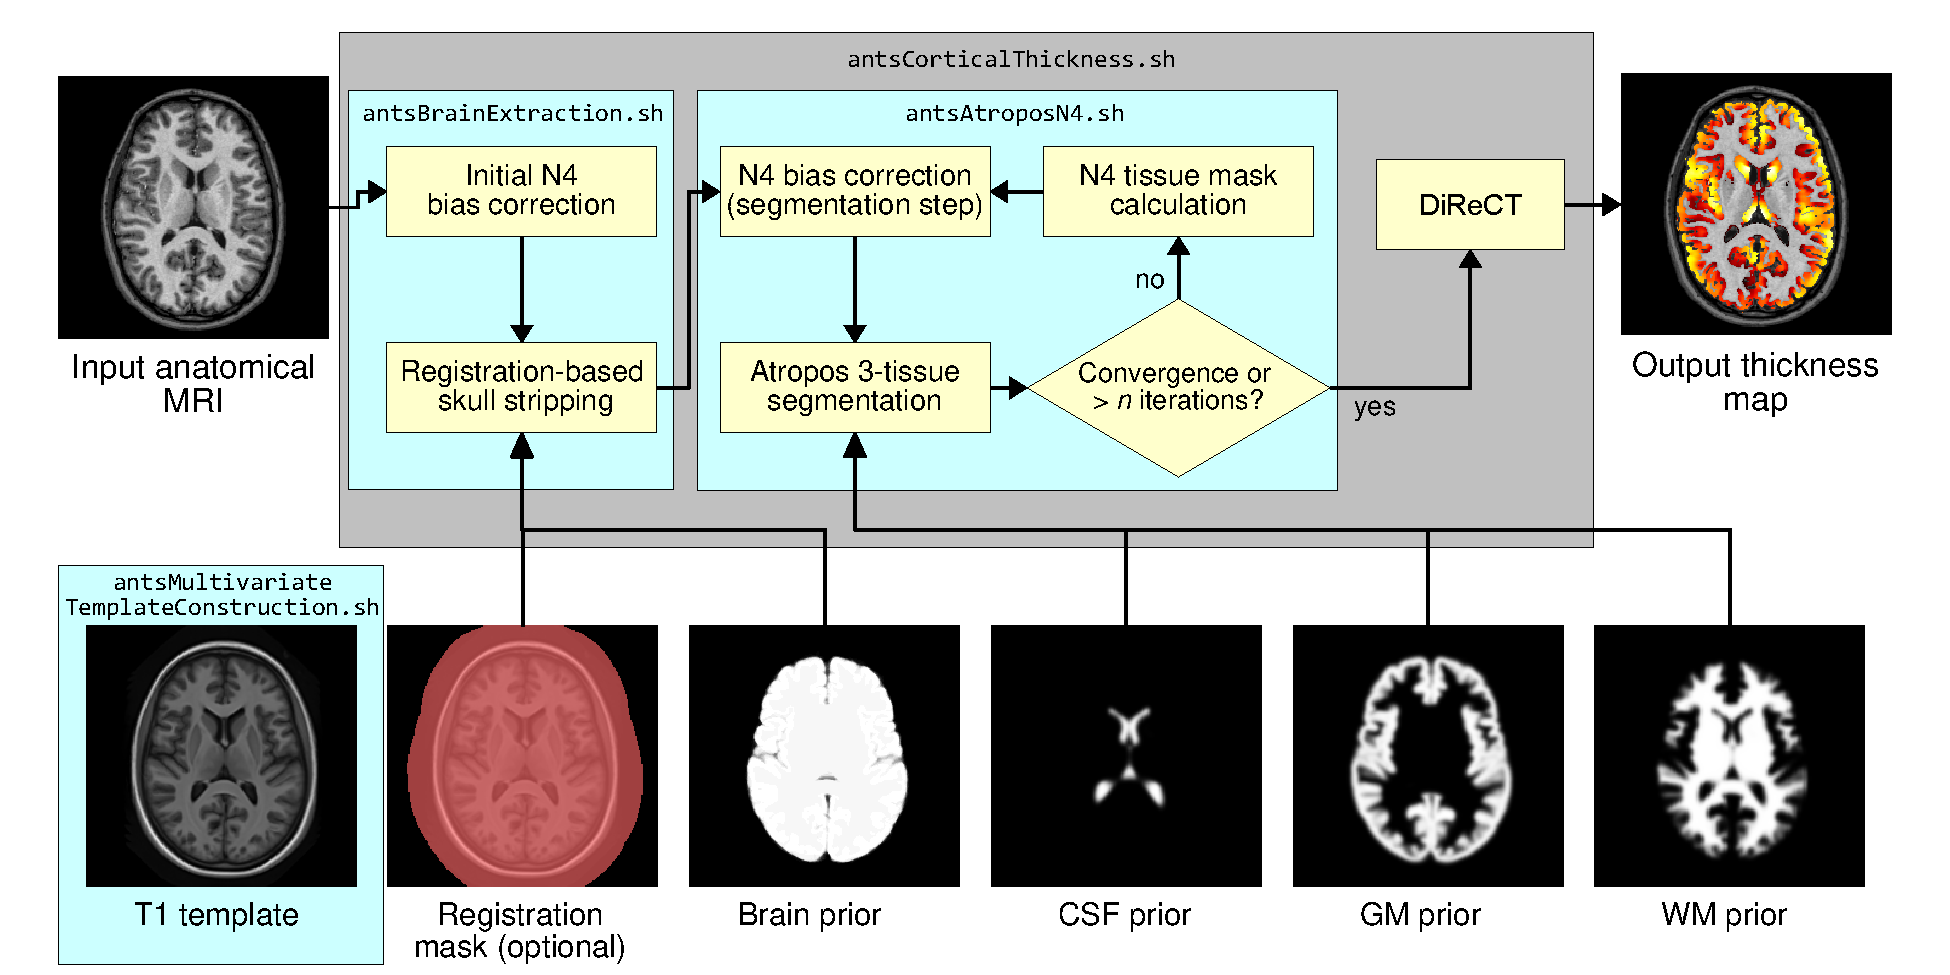
\includegraphics[width=180mm]{Figures/Kapowski_pipeline2.pdf}
  \caption{Illustration of the main components of the ANTs processing 
  workflow containing all elements for determining cortical thickness. 
  We also included the domain of operations for the selected scripts.
  Not shown are the probability maps for the brain stem and cerebellum
  priors.}
  \label{fig:pipeline}
\end{figure*}

\subsubsection{Anatomical template construction}

Registering (``normalizing'') images to a standard coordinate system
reduces intersubject variability in population studies.  Various
approaches exist for determining the normalization or coordinate space,
such as the selection of a pre-existing template based on a single individual
(e.g., the Talairach atlas \citep{Talairach1988}) or a publicly available average of multiple individuals
(e.g., the MNI \citep{Collins1994} or ICBM \citep{Mazziotta1995}
templates), or an average template constructed from the individuals under study.
The work of \cite{avants2010} explicitly models the geometric component of the 
normalized space during optimization to produce such mean templates.  Coupling the intrinsic symmetry of 
SyN pairwise registration \citep{avants2011} and an
optimized shape-based sharpening/averaging of the template appearance, Symmetric Group Normalization (SyGN) is a powerful framework for producing optimal population-specific templates.

The ANTs implementation of this technique is currently available as a shell script, 
{\tt buildtemplateparallel.sh}.  A generalized, multivariate version is also available as
{\tt antsMultivariateTemplateConstruction.sh}.  Both scripts are distributed as part of
 the ANTs software.  
The multivariate script permits the construction of multimodal templates
(e.g. T1-weighted, T2-weighted, proton density MRI and fractional anisotropy).
Both scripts accommodate a variety of computational resources
for facilitating template construction.  These computational resource possibilities include:
\begin{itemize}
  \item serial processing on a single workstation
  \item parallelized processing on a single workstation with multiple cores using \verb#pexec#%
  \footnote{http://www.gnu.org/software/pexec/pexec.1.html}
  \item parallelized processing using Apple's XGrid technology%
  \footnote{https://developer.apple.com/hardwaredrivers/hpc/xgrid\_intro.html}
  \item parallelized processing using Sun Grid Engine for cluster-based systems%
  \footnote{http://www.oracle.com/technetwork/oem/grid-engine-166852.html}
  \item parallelized processing using the Portable Batch System for cluster-based systems%
  \footnote{http://www.pbsworks.com/}
\end{itemize}

For this work, database-specific templates were used during cortical thickness pipeline
processing for both brain extraction and brain segmentation steps.  We used multivariate templates
because they had already been constructed for a previous study from the multimodal data sets,
not because they have been demonstrated to confer an advantage over univariate templates (i.e., T1-only)
for the proposed workflow.

\subsubsection{N4 bias field correction}

Critical to quantitative processing of MRI is the minimization of
field inhomogeneity effects which produce artificial low frequency 
intensity variation across the image.  Large-scale studies, such
as ADNI, employ
perhaps the most widely used bias correction algorithm, N3 \citep{sled1998}, 
as part of their standard protocol \citep{boyes2008}.

In \cite{tustison2010} we introduced an improvement of N3, denoted as
``N4'', which demonstrates a significant increase in performance and convergence behavior
on a variety of data. //REFERENCE NEEDED// This improvement is a result of an enhanced
fitting routine (which includes multi-resolution capabilities) and a modified optimization 
formulation.  For our workflow, the additional possibility of specifying
a weighted mask in N4 permits the use of a ``pure tissue'' probability map 
(described below)
calculated during the segmentation pipeline for further improvement of 
bias field estimation.  

N4 is used in two places during the individual subject processing (cf Figure
\ref{fig:pipeline}).  
It is used to generate an initial bias-corrected image for use in
brain extraction.  The input mask is created by adaptively thresholding 
the background from the foreground using Otsu's algorithm \citep{otsu1979}.
Following brain extraction, six-tissue (cerebrospinal fluid, cortical gray 
matter, white matter, deep gray matter, brain stem, and cerebellum)
segmentation involves iterating
between bias field correction using the current pure tissue 
probability map as a weight mask and then using that bias-corrected image
as input for the Atropos segmentation step (described below).

\subsubsection{Brain extraction}

\begin{figure*}
  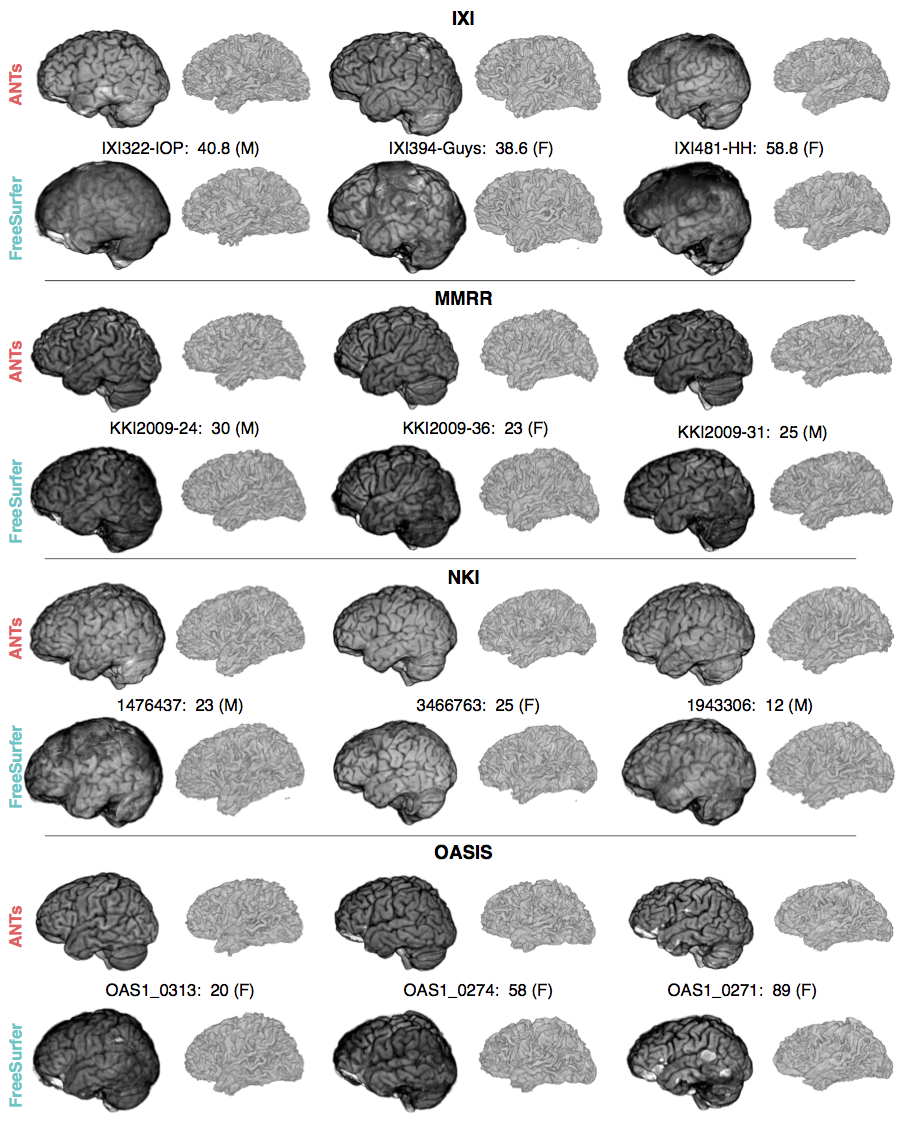
\includegraphics[width=180mm]{montage2.pdf}
  \caption{Representative sample of volume brain renderings from the four
  different cohorts (IXI = rows 1 and 2, Kirby = rows 3 and 4, 
  NKI = rows 5 and 6, Oasis = rows 7 and 8),
  illustrating the qualitative difference between ANTs and FreeSurfer 
  (``FS'') results, which are arranged top-and-bottom for each subject.  Each brain was rigidly
  registered to the Oasis template for rendering purposes.  With each subject
  we provide subject ID, age, and gender.
  }
  \label{fig:brainExtraction}
\end{figure*}

//MOST OF THE IMAGES COME FROM IXI.  I WOULD PREFER TWO ROWS DEVOTED TO EACH COHORT,
 WITH ANTS ABOVE AND FS BELOW (AND PERHAPS THE ID, ETC., SHOWN ONLY BETWEEN EACH PAIR OF IMAGES).//

Brain extraction using ANTs combines template building, high-performance
brain image registration, and Atropos segmentation with topological refinements.
An optimal template \cite{avants2010} is first constructed using structural MRI data
that is accompanied by corresponding anatomical labels (e.g., the LPBA40 data set).
//LPBA40 2008 SHATTUCK REFERENCE//
//PERHAPS YOU SHOULD REFER TO "OPTIMAL TEMPLATES" ABOVE//
Template construction iterates between estimating
the optimal template and registering each subject to the optimal template.
Thus, the construction produces the transforms necessary to warp each 
subject's labels to the template space.  We use these transformed labels
to create a probabilistic estimate of the brain mask for the template.
In this work, we perform the additional step of building separate templates
for each cohort and propagating the probabilistic mask to each cohort template
using registration of the T1-weighted templates (cf Figure \ref{fig:template}).
Further refinements include thresholding the warped brain probability map
at 0.5 and dilating the resulting mask with a radius of two.  Atropos is used
to generate an initial three-tissue segmentation estimate within the mask
region.  Each of the three tissue labels undergoes specific morphological  //"SPECIFIC"?  COULDN'T YOU SPECIFY THEM HERE?//
operations which are then combined to create a brain extraction mask for use 
in the rest of the cortical thickness workflow using the script {\tt antsBrainExtraction.sh}.  

In an evaluation study, we compared an earlier version of our extraction method
with publicly available brain extraction algorithms, including
AFNI's \verb#3dIntracranial#
\citep{ward1999}, FSL's \verb#BET2# \citep{smith2002}, FreeSurfer's
\verb#mri_watershed# \citep{segonne2004}, and BrainSuite
\citep{dogdas2005}. We demonstrated that our combined
registration/segmentation approach \citep{avants2010a} performed
with an accuracy comparable to FreeSurfer and a parameter-tuned version of BrainSuite.
Figure \ref{fig:brainExtraction} presents a visual comparison of results derived with
the current ANTs brain extraction method and results obtained using FreeSurfer.

\subsubsection{Atropos six-tissue segmentation}

//I THINK YOU SHOULD ADD COMMAS AFTER ALL OF YOUR LATIN ABBREVIATIONS LIKE "e.g.," and "i.e.,".
SOME PEOPLE ALSO PREFER TO ITALICIZE THESE AS WELL.//

In \cite{avants2011a} we presented an open source $n$-tissue segmentation software tool
(which we denote as ``Atropos'') that attempts to distill over 20 years of active research in this area,
in particular some of the most seminal work (e.g., \cite{zhang2001,ashburner2005}).
Specification of prior probabilities includes spatially varying Markov Random Field modeling, 
prior label maps, and prior probability maps typically derived from our template building 
process.  Additional
capabilities include handling of multivariate data, 
partial volume modeling \citep{shattuck2001}, a memory-minimization mode,
label propagation, a plug-and-play architecture for incorporation of novel likelihood models
which includes both parametric and non-parametric models for both scalar and tensorial
images, and alternative posterior formulations for different segmentation tasks.

Due to the important interplay between segmentation and bias correction,
we perform multiple N4 $\rightleftharpoons$ Atropos iterations.
In order to better integrate Atropos and N4, we use  
a pure tissue probability weight mask generated from the 
posterior probabilities derived from the segmentation 
step.  Given $N$ labels and the corresponding $N$
posterior probability maps $\{ P_1, \ldots, P_N\}$ produced
during segmentation, the N4 weight mask is 
created at each N4 $\rightleftharpoons$ Atropos iteration from
\begin{align}
  P_{pure\,\,tissue}(\mathbf{x}) = \sum_{i=1}^N P_i(\mathbf{x}) \prod_{j=1, j \neq i}^N \left( 1 - P_j(\mathbf{x}) \right).
\end{align}
One of the key insights of the original N3 development is the
observation that inhomogeneities cause the intensity values of
pure tissue peaks to spread in the intensity histogram as though
convolved with a Gaussian.  A core contribution of N3 is the
proposed corrective step of deconvolving the intensity histogram to
accentuate the tissue peaks, coupled with a spatial smoothing
constraint. The pure tissue probability mask
weights more heavily the voxels corresponding to pure tissue 
types (as determined by the segmentation) during the deconvolution process 
while minimizing the contribution of regions such as the gray/white matter 
interface where peak membership is ambiguous. 

Atropos enables prior knowledge to guide the
segmentation process where template-based priors are integrated into the optimization
with a user-controlled weight.  Modulating the likelihood and prior contributions
to the posterior probability is essential for producing adequate segmentations.
Atropos weights the likelihood and priors according to
$P(x|y) \propto P(y|x)^{1-\alpha}P(x)^{\alpha}$
where $\alpha$ is a user-selected parameter which weights the tradeoff between the likelihood and priors terms.
In this work, we chose a weighting of $\alpha = 0.25$ 
based on our extensive experimentation with different parameter weights.
//WHAT DATA WERE THESE EXTENSIVE EXPERIMENTS RUN ON? DID THEY INTERSECT WITH THE DATA IN THIS STUDY?//

Since cortical thickness estimation only requires the cortical gray
and white matter, the deep gray and white matter
(both labels and posterior maps) are combined to form a single
``white matter'' set.  This white matter set and the cortical
gray matter are the only results from the segmentation
step that are used by the DiReCT algorithm (described below).


\subsubsection{DiReCT (aka KellySlater/KellyKapowski) cortical thickness estimation}

//I WOULD REMOVE ALL THE OTHER NAMES IN THE SUBSUBSECTION HEADER, SINCE YOU LIST THEM IN THE TEXT BELOW.//

DiReCT was introduced 
in \cite{das2009} and was made available in ANTs as the program \verb#KellySlater#.
Since then several improvements have been made and incorporated into the program
\verb#KellyKapowski#.%
\footnote{
Traditional academic discourse encountered in the published literature
rarely contextualizes peculiarities such as algorithmic nomenclature.
We briefly mention that
this //NAME// was the source of a rare disagreement between the first and last authors
based, as many disagreements are, on a simple misunderstanding and not an
affronting existential statement concerning a certain favorite sitcom
of the first author's youth. 
}

//LOVE THE ABOVE FOOTNOTE!//

The more recent implementation has made numerous advances, including:
it is multi-threaded, written in rigorous ITK coding style //REFERENCE//, and
has been made publicly available through ANTs, complete with a unique user
interface design developed specifically for ANTs tools.

//WHAT USER INTERFACE?//

\subsection{Public data resources}

The above pipeline was run on four publicly available data sets:
IXI, Kirby, NKI, and Oasis.  //OASIS?//
In addition, we used a subset of the MindBoggle-101 data%
\footnote{
http://mindboggle.info/data.html
} 
labeled using the 
Desikan-Killiany-Tourville (DKT) protocol \citep{klein2012} to define the
regions of interest (ROI).
All five data sets are described below.

\subsubsection{MindBoggle-101 data for ROI definitions}

In \cite{klein2012} the authors proposed the DKT cortical labeling protocol---a modification of the
popular Desikan-Killiany protocol \cite{desikan2006} to improve cortical labeling
consistency and to improve FreeSurfer's cortical classification of 31 cortical regions per hemisphere,
listed in Table \ref{table:dkt_labels}.
For the latter, forty manually labeled brains were used to construct the DKT40 Gaussian classifier atlas,
which is now bundled with current versions of FreeSurfer and
used to automate anatomical labeling of MRI data.
Since the regional thickness values generated by FreeSurfer follow this protocol,
these anatomical labels provide a common standard for comparison between ANTs and FreeSurfer.

The work of \cite{klein2012} also resulted in a publicly available set of
manually edited labels following the DKT protocol in 101
T1-weighted  brain images from different sources, including a subset of 20 images
from the Oasis data set.  These 20 images are used in the ANTs
multi-atlas label propagation \cite{wang2013} step that defines the volumetric regions for each subject.
The parameters for this step may be found in the {\tt antsMalfLabeling.sh} script, which is also
distributed with the ANTs toolkit.  //CAN'T YOU LIST THE PARAMETERS HERE?//
Cortical thickness values are averaged within each labeled region for each subject using only
the non-zero voxels from the cortical thickness map.
//DO YOU USE THE MANUAL LABELS IN THE MINDBOGGLE-101 SET SO THAT REVIEWERS CAN'T
COMPLAIN ABOUT THE MULTI-ATLAS LABELING STRATEGY?//

\begin{table}
\centering
\begin{tabular*}{0.475\textwidth}{@{\extracolsep{\fill}} l l}
\toprule
  1) caudal anterior cingulate & 2) caudal middle frontal \\
  3) cuneus & 4) entorhinal \\
  5) fusiform & 6) inferior parietal \\
  7) inferior temporal & 8) isthmus cingulate \\
  9) lateral occipital & 10) lateral orbitofrontal \\
  11) lingual & 12) medial orbitofrontal \\
  13) middle temporal & 14) parahippocampal \\
  15) paracentral & 16) pars opercularis \\
  17) pars orbitalis & 18) pars triangularis \\
  19) pericalcarine & 20) postcentral \\
  21) posterior cingulate & 22) precentral \\
  23) precuneus & 24) rosterior anterior cingulate \\
  25) rostral middle frontal & 26) superior frontal \\
  27) superior parietal & 28) superior temporal \\
  29) supramarginal & 30) transverse temporal \\
  31) insula & {} \\  
\bottomrule
\end{tabular*}
\caption{The 31 cortical labels (per hemisphere) of the DKT atlas.  }
\label{table:dkt_labels}
\end{table}

//WHAT IS WITH THE WEIRD NUMBERING IN THIS TABLE -- WHY NOT SIMPLY LIST UP-TO-DOWN?//

\subsubsection{Public data for thickness estimation evaluation}

\begin{figure}
  \centering
  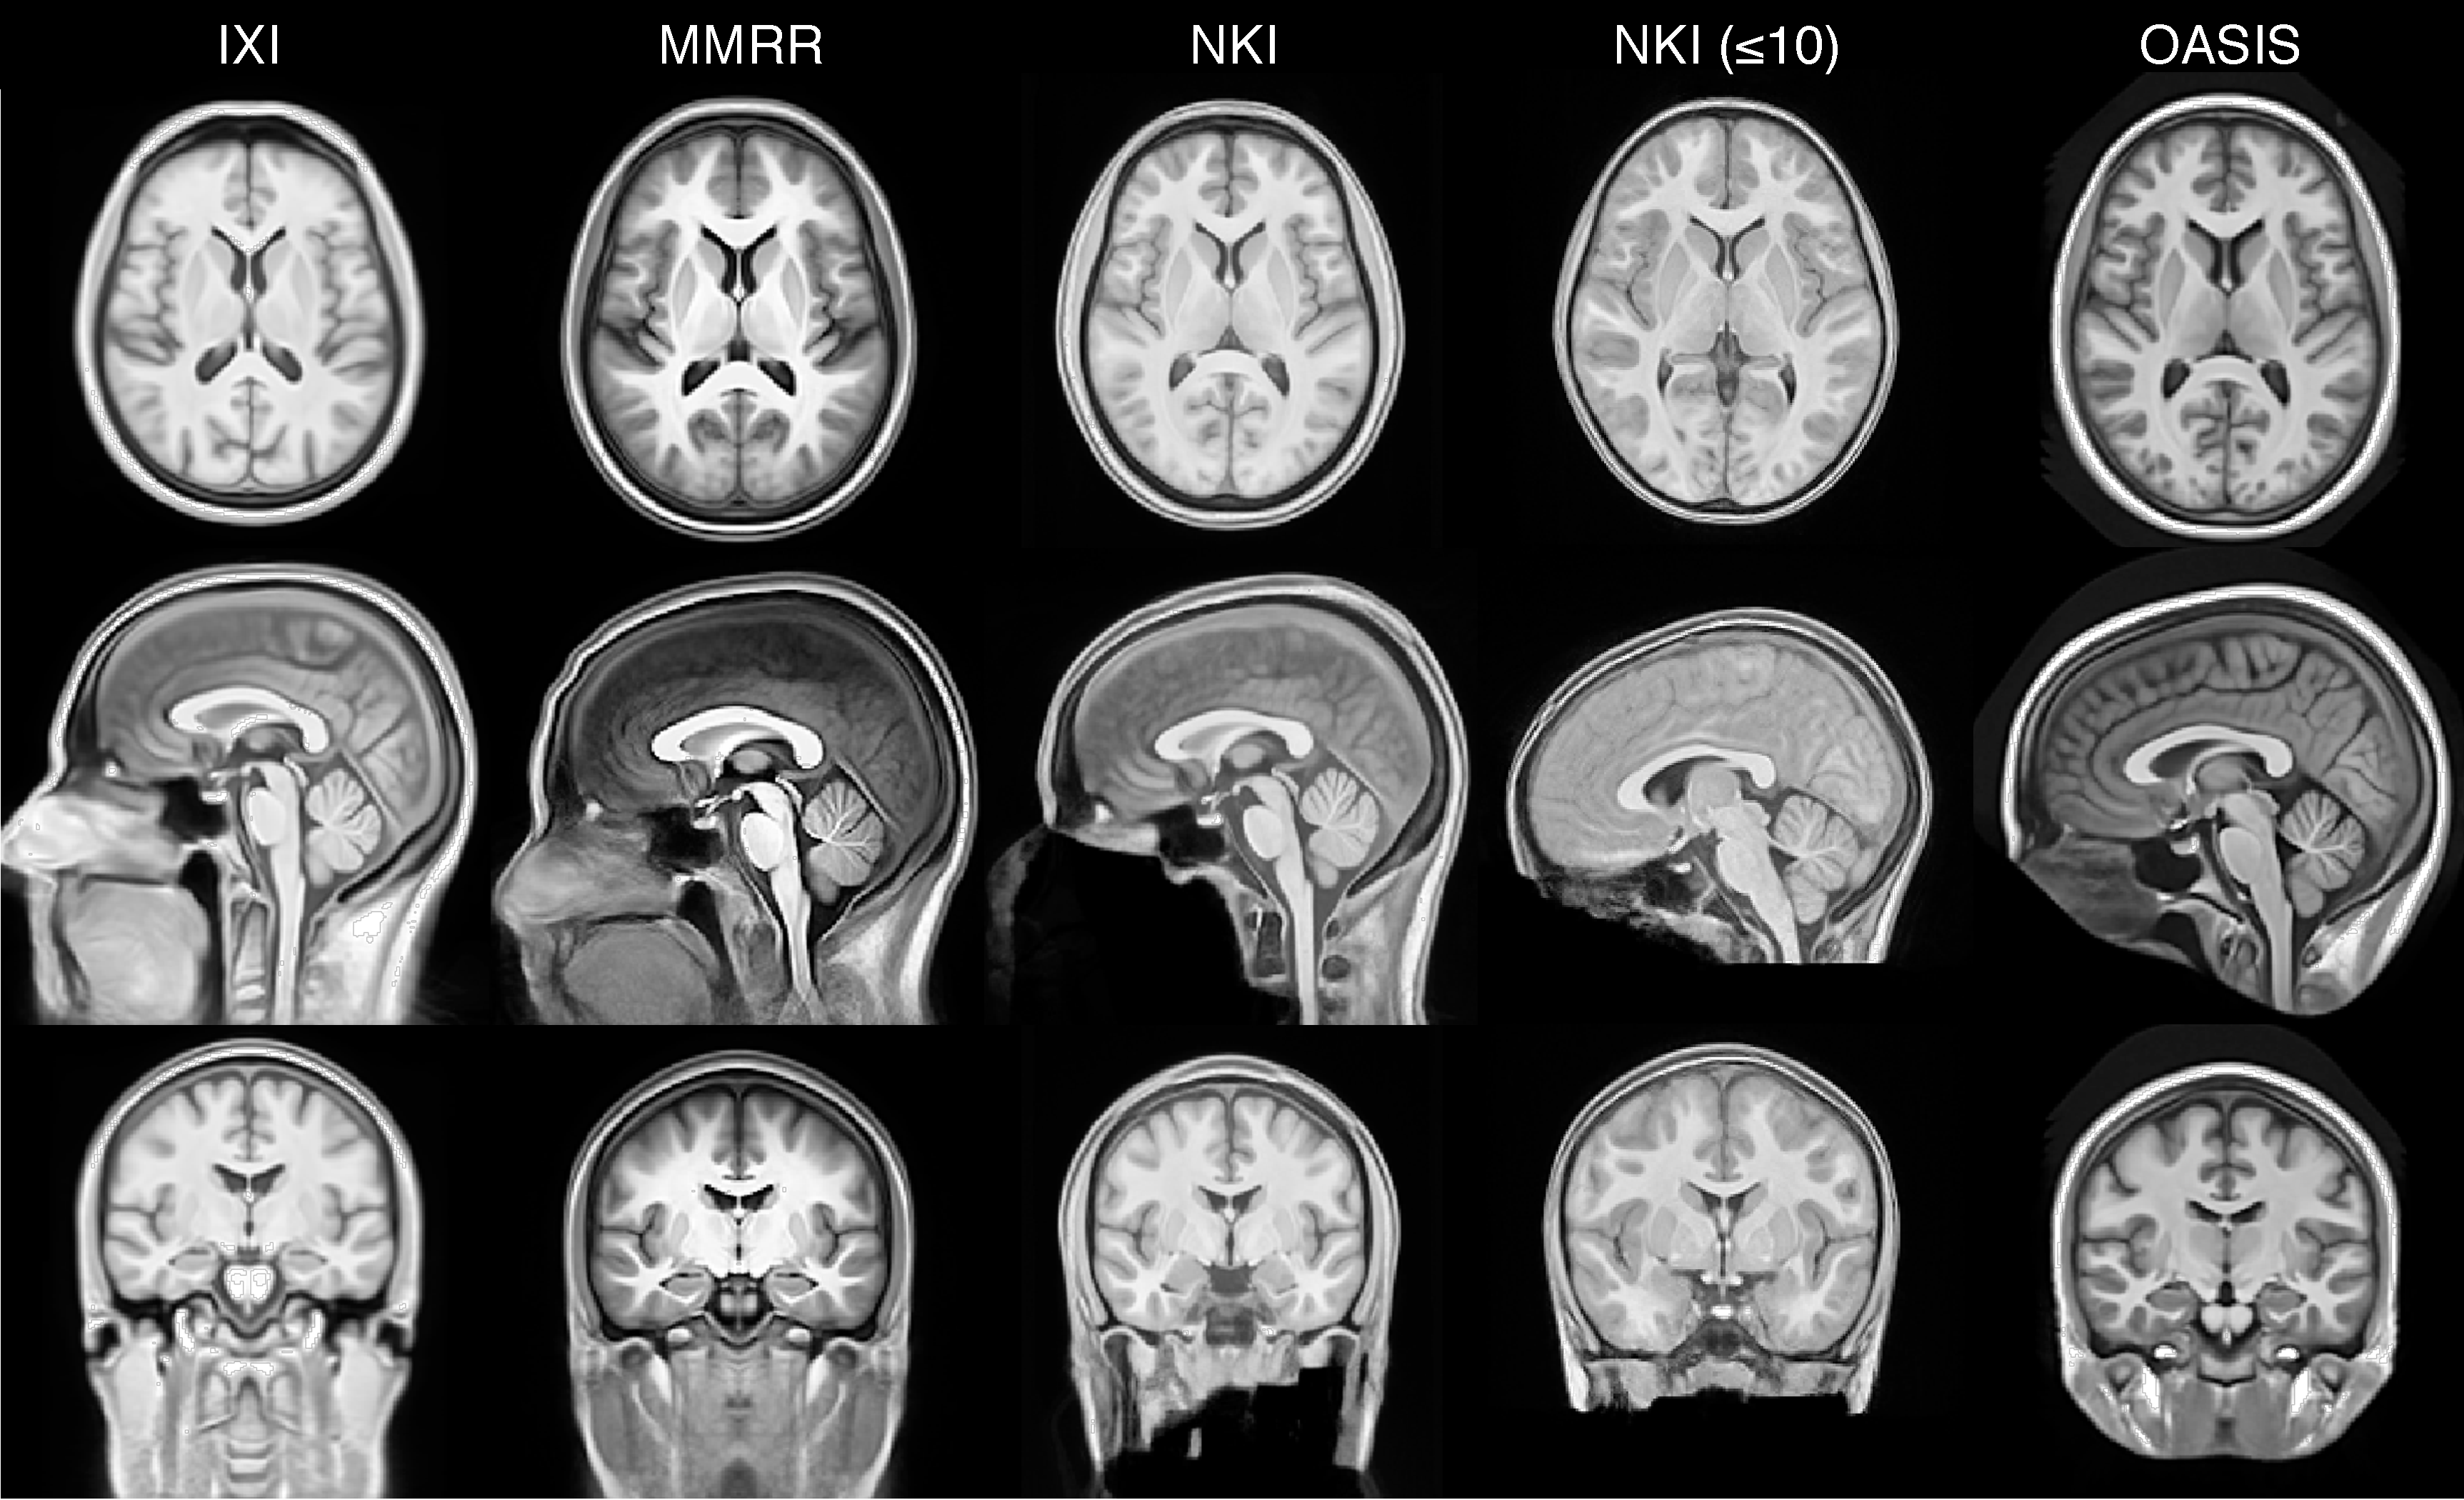
\includegraphics[width=90mm]{Figures/templates.pdf}
  \caption{Population-specific templates for each of the four public data sets used
  for cortical thickness 
  estimation. These templates were generated using the script {\tt antsMultivariateTemplateConstruction.sh}.
  The benefit of using such population-specific templates is obvious when one sees the variability in
  acquisition and data preparation (e.g. defacing protocols).
  }
  \label{fig:template}
\end{figure}

We apply //PAST TENSE?// the same pipeline to diverse publicly available data sets collected
from multiple sites and with a mixture of 3T and
1.5T T1 brain images.  Subjects in this data set  //I CHANGED ALL "DATASET" TO "DATA SET" TO BE CONSISTENT. CHOOSE ONE OR THE OTHER//
span the age range from 4 to 96 years old.  This strategy tests robustness to
variation in head position, brain shape, defacing, image contrast, inhomogeneity, imaging
artifacts, and the broad variation in extracerebral tissue.  Failure
can occur in initial brain extraction, segmentation, registration, or
bias correction, any of which will lead to an inaccurate cortical
thickness measurement.                           

In total, we processed 1,205 T1-weighted images from four different
public data sets to obtain cortical thickness maps.
Below we describe the four data sets:
                                          
\paragraph{IXI}
Initially, we processed 581 T1-weighted images from the IXI%
\footnote{
http://biomedic.doc.ic.ac.uk/brain-development/
}
 data set, but only 563 subjects
(313 females, 250 males) were included in the post processing analysis due to 
missing demographic information, which would have prevented an accurate estimate of
the age at the time of image acquisition.  These data were
imaged at three sites 
with several modalities acquired (T1-weighted, T2-weighted, proton density, magnetic 
resonance angiography, and diffusion tensor imaging).  The 
database also includes demographic information such as date of birth, date
of scan, weight,
height, ethnicity, occupation category, educational level, and marital status.


//WHY USE "KIRBY" AS OPPOSED TO MMRR?//

\paragraph{Kirby}
The Multi-Modal MRI Reproducibility Resource%
\footnote{
http://www.nitrc.org/projects/multimodal/
}, 
or more informally, the Kirby
data set, was originally described in \cite{landman2011} consisting of 
21 subjects (10 females, 11 males) and features a rich set of modalities, as well as repeated scans.

\paragraph{NKI}
In support of open science, the 1,000 Functional Connectomes Project%
\footnote{ 
http://fcon\_1000.projects.nitrc.org
}
was initiated on December 11, 2009 by various members of the MRI community
seeking to form collaborative partnerships among imaging institutions for
sharing well-documented multimodal image sets accompanied by phenotypic data.
One such contribution is the Nathan Klein Institute (NKI)/Rockland sample,
consisting of 186 T1-weighted
images (87 females, 99 males).%
\footnote{
Downloaded on September 22, 2012.
}

\paragraph{Oasis}
The initial Open Access Series of Imaging Studies (OASIS)%
\footnote{
http://www.oasis-brains.org/
}
data set consisted of 433 T1-weighted images.  We processed all of these,
but 100 were excluded from our analysis due to probable Alzheimer's
disease ($CDR > 0$) and an additional 20 repeat scans were excluded,
 resulting in 313 individual subject scans included in the normal group statistical
analysis (118 males, 195 females).
Ages were between 18 and 96 and  
all subjects are right-handed.  
%Additional processing is included
%with the distribution including bias corrected and segmented images
%(gray, white and CSF matters).  


\begin{figure}
  \centering
  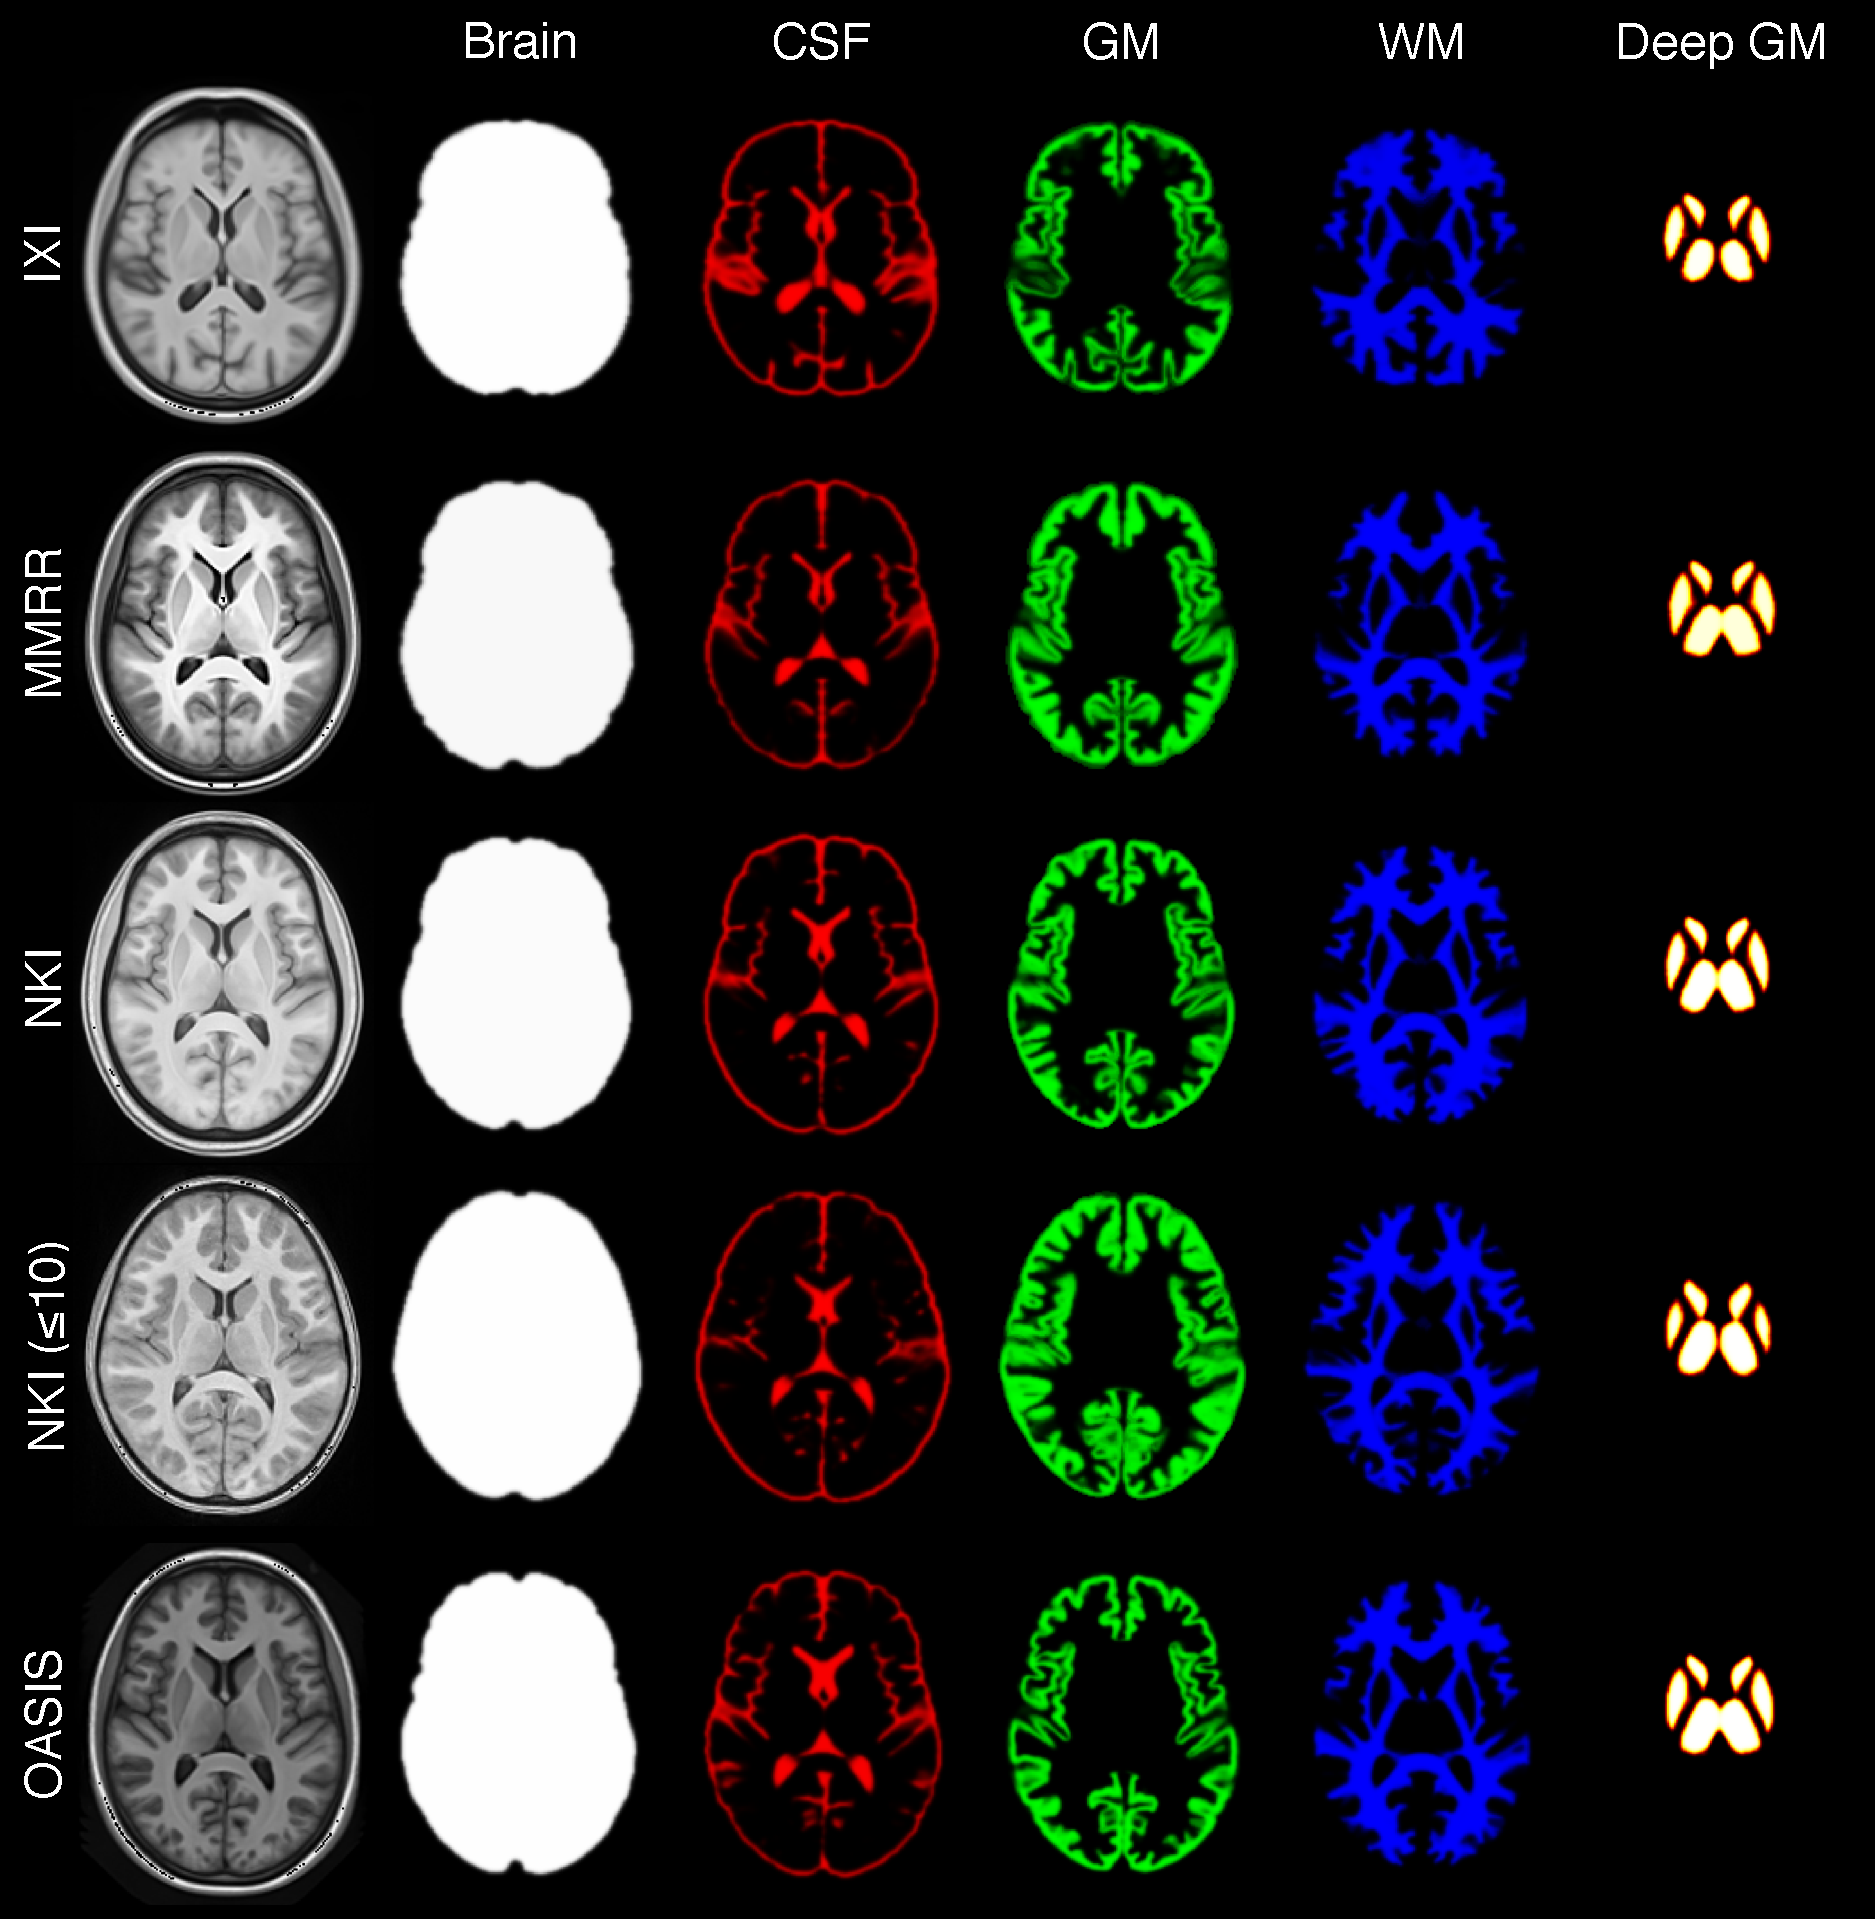
\includegraphics[width=90mm]{Figures/templateProbabilityMasks.pdf}
  \caption{Axial slices from each of the five T1 templates including the corresponding
  probability masks used for brain extraction and brain tissue segmentation.  Not shown
  are the prior probability maps for brain stem and cerebellum regions.
  }
  \label{fig:templateMasks}
\end{figure}


\subsection{Processing miscellany}

Given the documented variability in FreeSurfer results with version and
operating system \cite{gronenschild2012} (as we would expect with our own ANTs pipeline),
all data was processed using the same ANTs and FreeSurfer versions on the same 
hardware platform.  Processing was performed using the Linux (CentOS release 6.4) 
cluster at the University 
of Virginia%
\footnote{
http://www.uvacse.virginia.edu/
}
using single-threading with a maximal requested memory footprint of 8 gb for ANTs 
and 4 gb for FreeSurfer.  The development version of ANTs was used for processing 
(git commit tag: 69d3a5a6c7125ccf07a9e9cf6ef29f0b91e9514f, date Dec. 11, 2013).  
FreeSurfer version 5.3 x86\_64 for CentOs was downloaded 
on 5 December, 2013 (``freesurfer-Linux-centos6\_x86\_64-stable-pub-v5.3.0'', release
date: 15 May, 2013). 




\begin{figure*}[htb]
  \centering
  \begin{tabular}{c}
  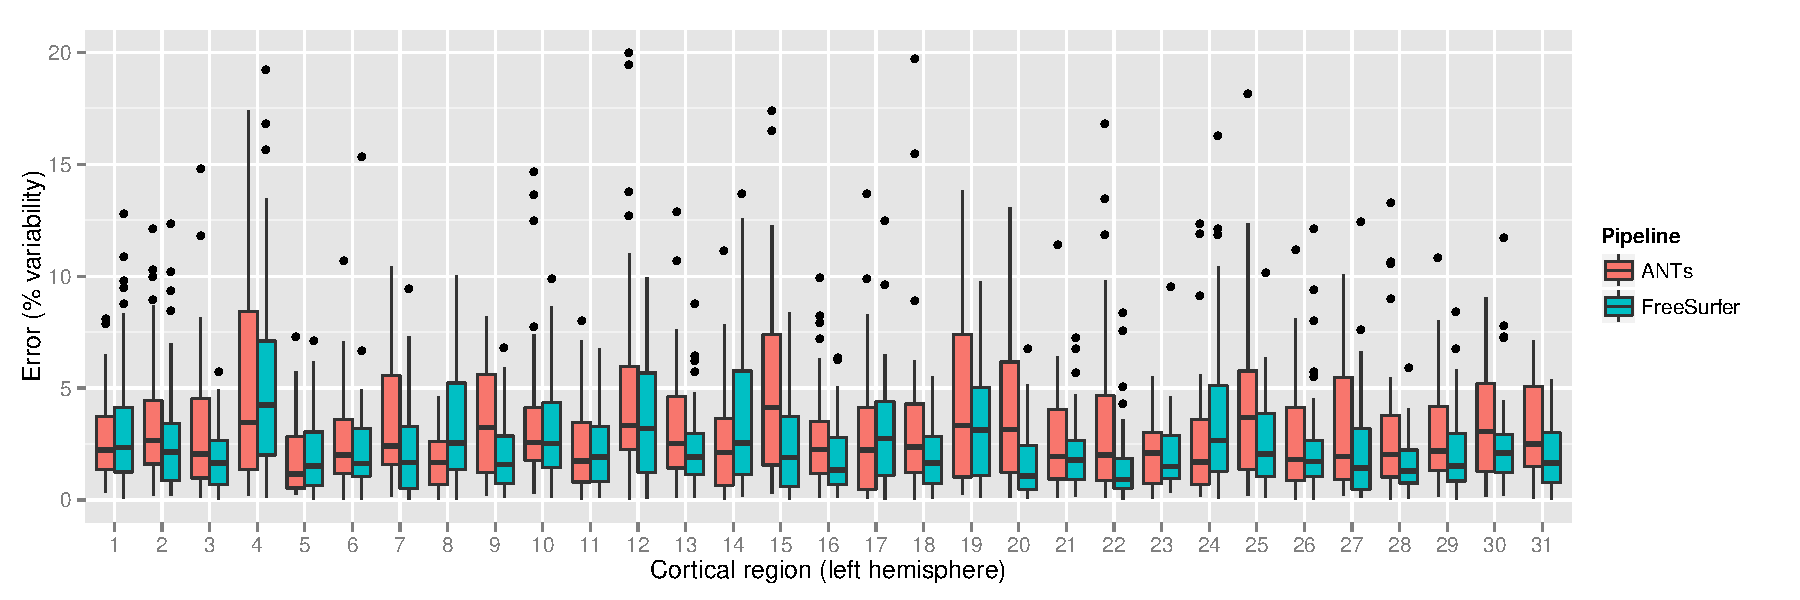
\includegraphics[width=180mm]{repeatabilityLeft.pdf} \\
  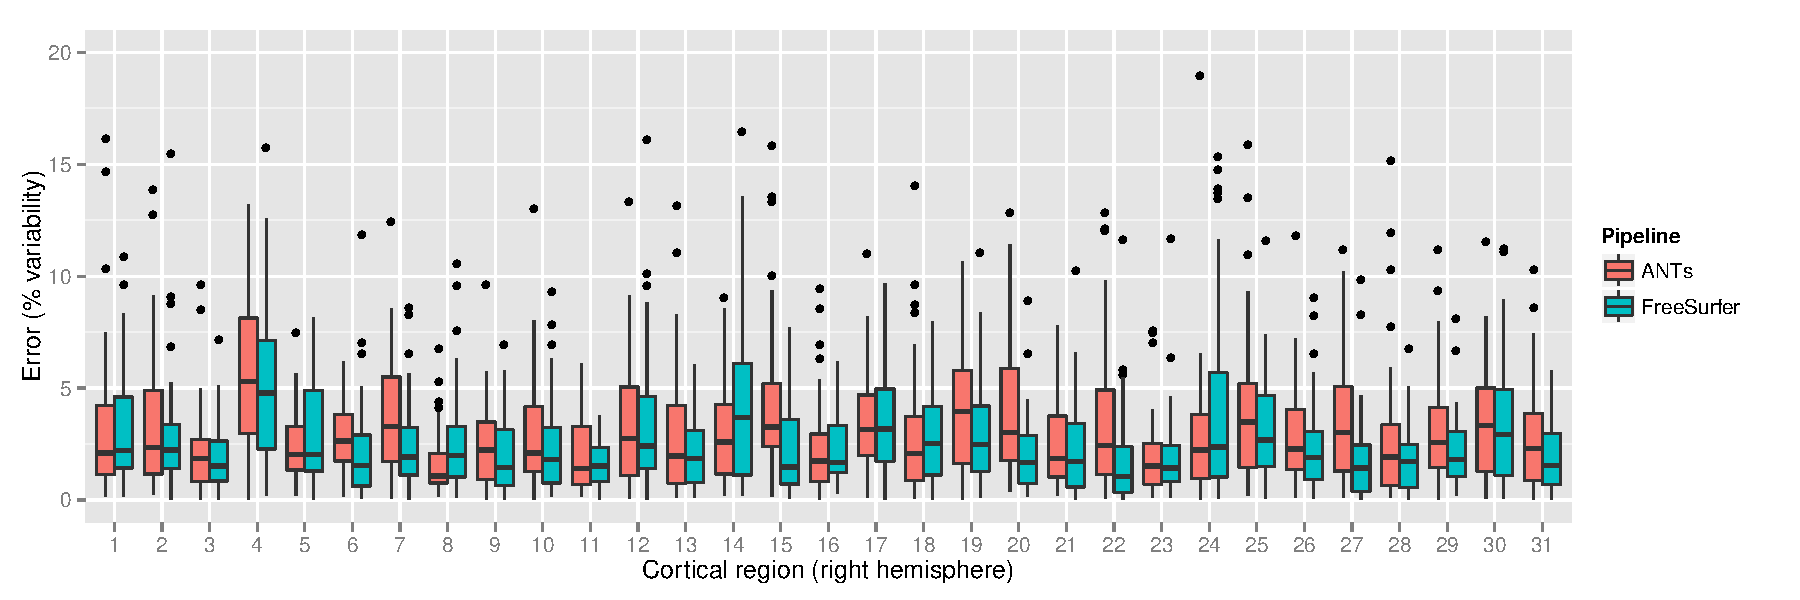
\includegraphics[width=180mm]{repeatabilityRight.pdf}
  \end{tabular}
  \caption{Percent error variability for both ANTs and FreeSurfer pipelines 
           over the left and right hemispheres of both the MMRR and OASIS
           data subsets within the 62 regions defined by the
           Desikan-Killiany-Tourville atlas.  Both methods demonstrate good repeatability
           qualities.
           }
  \label{fig:repeatability}
\end{figure*}


\section{Evaluation}
Traditional assessment approaches, such as manual
labeling, are inadequate for evaluating large-scale performance.  
We therefore sought to minimize failure rate, quantify the repeatability of cortical
thickness measures, and
determine whether the ANTs pipeline reveals biologically plausible relationships
between the cortex, gender,%
\footnote{
We recognize the distinction often made between ``sex'' and ``gender'' 
(cf {\tt http://www.who.int/gender/whatisgender/en/}).
As the demographic information collected during the course of the imaging studies 
is presumably self-reported, we assume that most self-identify in terms of 
gender and, therefore, use the term ``gender'' in data
descriptions.
}
and age and how its performance compares
to the current de facto standard of FreeSurfer-derived thickness estimation.
Collectively, these surrogate
measurements allow us to establish data-derived relative performance standards.
Additionally, for completeness, we include timing results as that factors into
usability.

\subsection{Repeatability}%

Repeat scans of 40 subjects (20 MMRR subjects and 20 OASIS subjects) were 
used to determine the repeatability of regional cortical thickness 
measurements, $T$.  Similar to the reproducibility 
assessment given in \cite{jovicich2013}, we
demonstrate this in terms of the percent variability error:
\begin{align}
\varepsilon = \frac{|T_{scan} - T_{rescan}|}{0.5 \times (T_{scan} + T_{rescan})}.
\end{align}
Comparison of the ANTs and FreeSurfer percent variability errors for the 62 DKT 
regions for both the OASIS and MMRR scan-rescan data sets
are given in Figure \ref{fig:repeatability}.  Although the variance is slightly greater 
for the set of ANTs measurements, statistical testing per cortical region 
(two-tailed paired t-test, corrected using false discovery rate) did not indicate 
non-zero mean differences for either approach for any region.

We also calculated the intraclass correlation coefficient 
(``ICC(2,1)'' in the notation of \cite{shrout1979}) to assess 
scan/rescan reliability. The ANTs thickness pipeline produced an 
ICC value of 0.98 and the FreeSurfer thickness pipeline yielded
an ICC value of 0.97, indicating good scan/rescan reliability for
both ANTs and FreeSurfer.

\subsection{Age prediction assessment}

Despite good repeatability with both ANTs and FreeSurfer, such measures
do not provide an assessment of accuracy or even relative utility.  For example, 
strong priors can yield good repeatability measures but potentially at the expense 
of data fidelity thus compromising the quality of models (statistical or otherwise) 
built from such results.  Given that ground truth is not available for 
these data nor for the many studies looking at brain
morphology, an indirect method (or set of methods) is required for
determining the quality of thickness estimation.

Previous research has used predictive modeling for comparing cortical
thickness algorithms.  For example, in \cite{clarkson2011}, classification
of healthy, semantic dementia, and progressive non-fluent aphasia categories
using regional cortical thickness values was used to determine the predictive
modeling capabilities of different cortical thickness processing protocols in 
101 subjects. However, differential diagnosis of dementia 
\cite{neary2005} is not as straightforward as obtaining a subject's age
or gender and regressing that against cortical thickness; the latter constitute biological
relationships that have been well-studied and reported in the literature.

\begin{figure}[htb]
  \centering
  \begin{tabular}{c}
  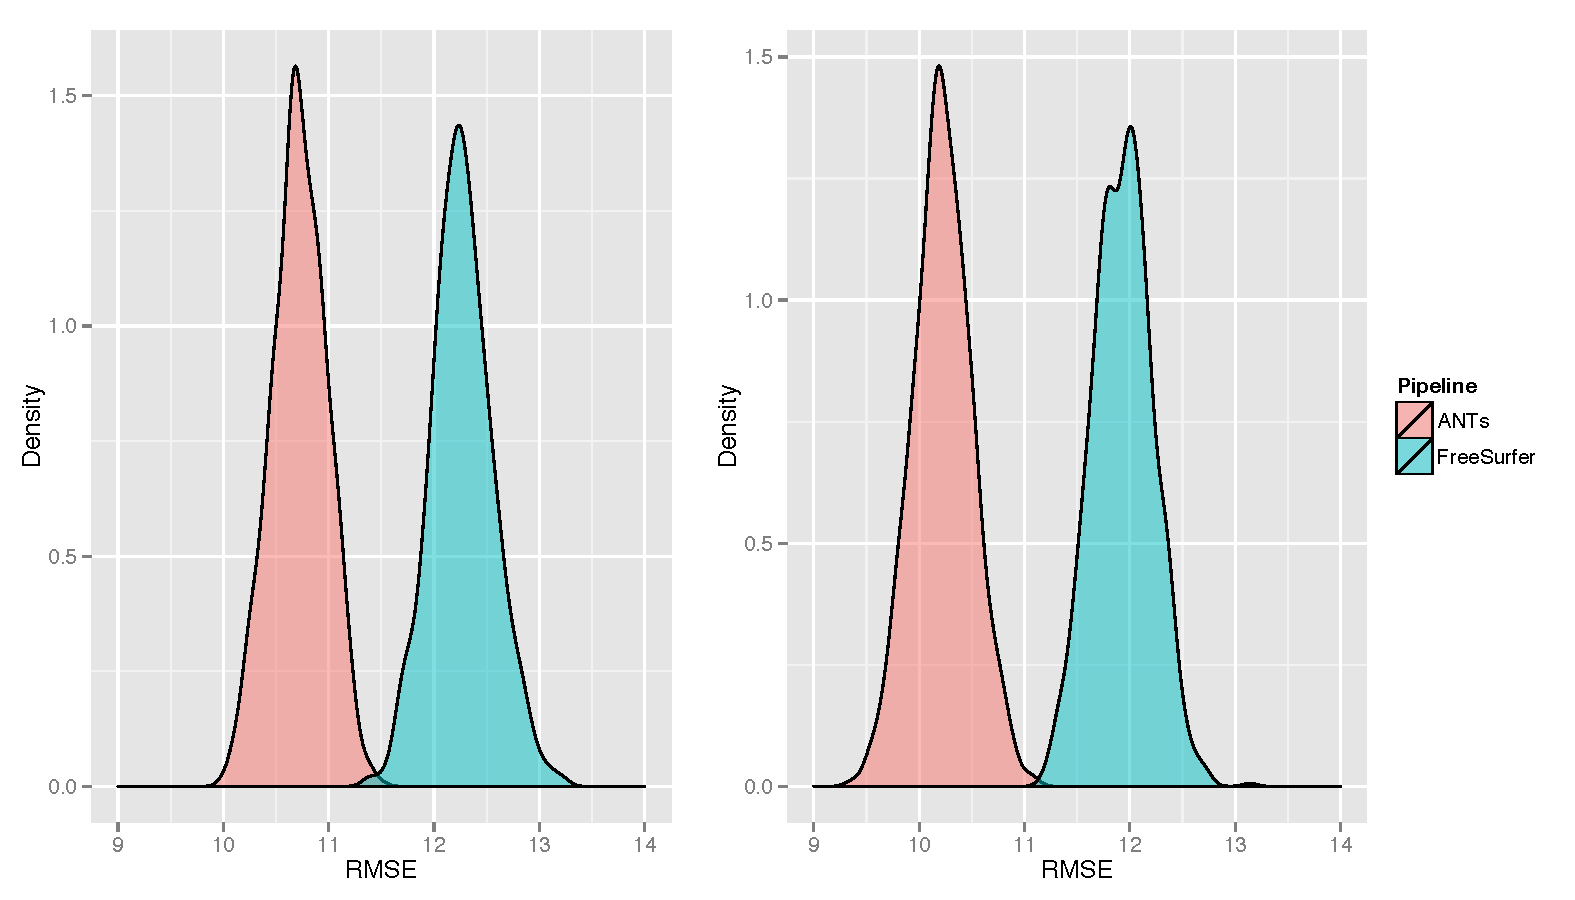
\includegraphics[width=85mm]{agePrediction.pdf} \\
  \end{tabular}
  \caption{Age prediction RMSE distributions of linear (left) and random forest (right)
           models for the ANTs- and FreeSurfer-derived thickness values.  For both prediction
           models ANTs RMSE error is lower.
           }
  \label{fig:agePrediction}
\end{figure}


For our first assessment, we modeled age versus regional cortical thickness values 
to determine which framework produces better predictive thickness estimates.  We first
subdivided the thickness data into training and testing subsets with an even split
between the two subsets.%
\footnote{
We tried various training proportions between 10 and 90\% (in increments of 10\%)
to see if that had an effect on relative performance for both age and 
gender prediction comparisons. Although age predictive capabilities for 
both pipelines showed improvement (gender prediction was mostly unaffected), 
the relative outcomes were the same.  
}
We then used the training data to create two models for each pipeline:
1) standard linear regression
and 2) random forests (a non-parametric machine learning technique) \cite{breiman2001},
for estimating age from both ANTs and FreeSurfer thickness values in the testing data.  

The formula (in the notation of \cite{wilkinson1973}) for the linear model is
\begin{align}
  AGE \sim VOLUME + \sum_{i=1}^{62} T(DKT_{i})*GENDER
\end{align}
where $T(DKT_{i})$ is the average thickness value in region $DKT_{i}$.
Similarly, the random forest 
model was specified as a combination of all terms
using the {\tt randomForest}%
\footnote{
http://cran.r-project.org/package=randomForest
}
package in R with the default settings and 200 trees.

In order to ensure a fair comparison, the procedure described above consisting
of training and testing steps was performed for $n = 1000$ permutations to elicit a 
performance distribution which we measure using the relative mean square
error (RMSE):
\begin{align}
  RMSE = \sqrt{\frac{\sum \left(AGE_{true} - AGE_{predicted} \right)^2}{N}}.
\end{align}
The resulting distributions are illustrated in Figure \ref{fig:agePrediction}
with the linear model results displayed on the left and random forest results
on the right.  The RMSE value was lower with ANTs thickness values for both 
models with the ANTs-based random forest predictions performing the best.  
Mean RMSE values are provided in Table \ref{table:agePrediction}.

\begin{table}
\caption{Mean RMSE for age prediction (in years).}
\label{table:agePrediction}
\centering
\begin{tabular*}{0.4\textwidth}{@{\extracolsep{\fill}} l c c}
\toprule
{} &        {\bf Linear}  &  {\bf Random Forest} \\
\midrule
ANTs &       12.2   &       10.3 \\
FreeSurfer & 13.9   &       12.3 \\
\bottomrule
\end{tabular*}
\end{table}


\subsection{Gender prediction assessment}

\begin{figure}[htb]
  \centering
  \begin{tabular}{c}
  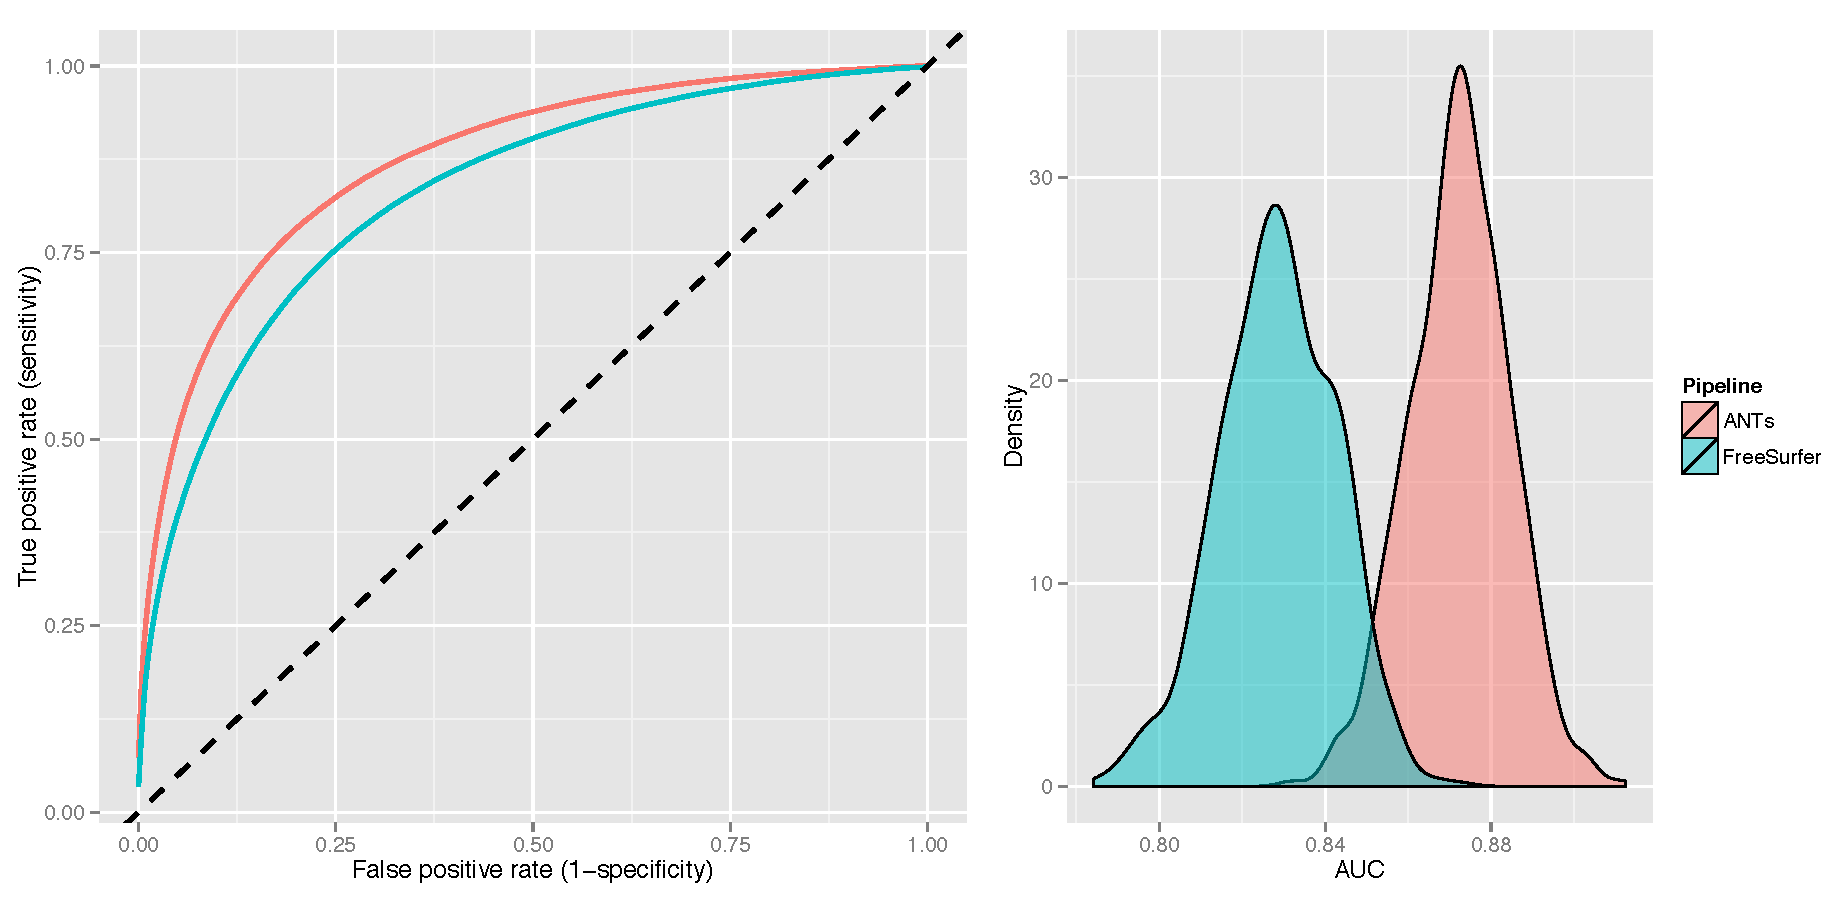
\includegraphics[width=85mm]{genderPrediction.pdf}
  \end{tabular}
  \caption{Average ROC curve and corresponding AUC distributions
  for gender prediction using ANTs and FreeSurfer thickness values.
  Values were averaged for 1000 permutations resulting in mean
  values of ANTs$_{AUC} =0.83$ and FreeSurfer$_{AUC} =0.78$.
  }
  \label{fig:genderPrediction}
\end{figure}

We also performed a similar prediction assessment using gender
as the regressand.   The binomial generalized linear model is
\begin{align}
  GENDER \sim VOLUME + \sum_{i=1}^{62} T(DKT_{i})*AGE
\end{align}
where $T(DKT_{i})$ is the average thickness value in region $DKT_{i}$.
We then characterized performance using a ROC curve for both methods 
(see Figure \ref{fig:genderPrediction}) where we averaged over 1000
permutations.  The mean area under the curve (AUC) for
both methods was also quantified with values of ANTs$_{AUC} =0.83$ and 
FreeSurfer$_{AUC} =0.78$.

   

\subsection{Computation time}

\begin{figure}[htb]
  \centering
  \begin{tabular}{c}
  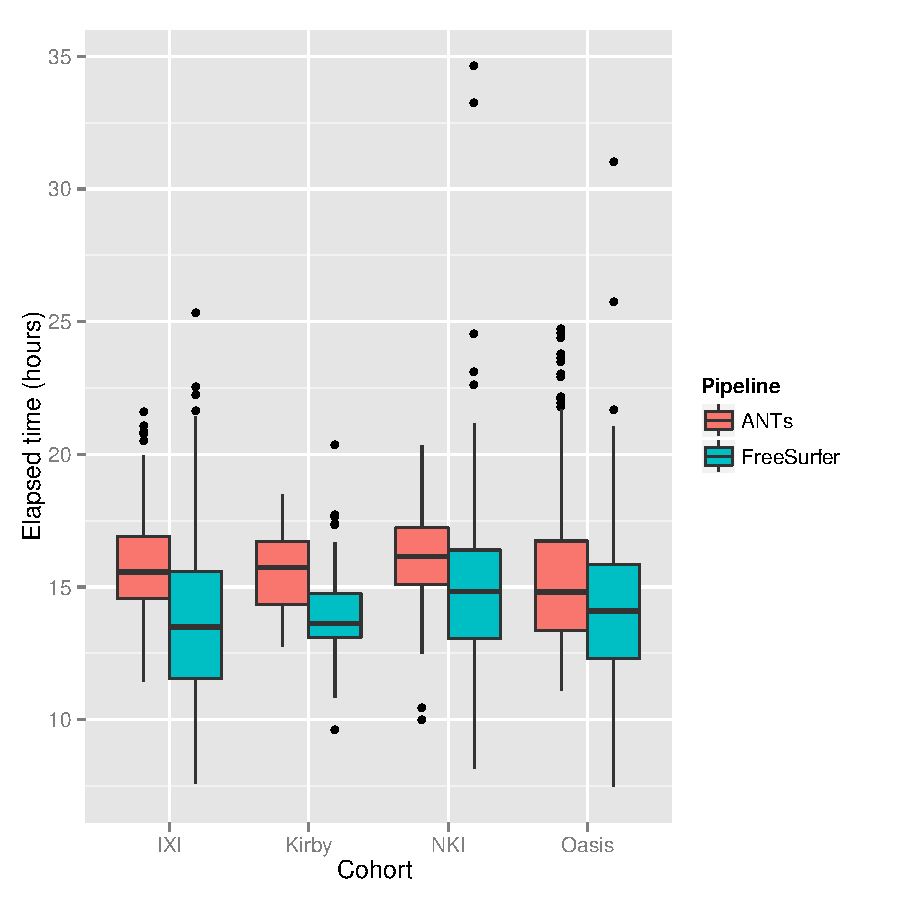
\includegraphics[width=90mm]{Times.pdf}
  \end{tabular}
  \caption{Elapsed time across data sets for ANTs and 
           FreeSurfer processing.  Averaged over all cohorts, ANTs required $15.7 \pm 2.0$ hours per subject and FreeSurfer required $14.1 \pm 2.9$ hours per subject.
           }
  \label{fig:times}
\end{figure}

All images underwent the ANTs and FreeSurfer pipeline processing 
using the computational cluster at the University of Virginia.  
Processing times varied approximately between 10--20 hours per subject
for both pipelines for the entire cortical thickness estimation procedure
although ANTs processing, on average, took slightly longer (cf Figure \ref{fig:times}).  Averaged over all cohorts, ANTs required 
$15.7 \pm 2.0 $ hours per subject and FreeSurfer required $14.1 \pm 2.9$ hours per subject.

The propagation of the DKT labels to each subject using label fusion as described earlier
was performed in parallel and took anywhere between 40 and 80 hours per 
subject for 16 serial image registrations and application of the joint label fusion algorithm \citep{wang2013}. For each subject, 20 atlas registrations are used to generate the labeling 
for that subject.  Therefore to do the MALF labeling for the entire cohort, approximately 
$1200 \times 20 = 24000$ registrations were required.  The {\tt antsMalfLabeling.sh} script
mentioned earlier parallelizes
the registration component which decreases the time for parallel computation platforms.
 
 
 


%
\section{Discussion}
In the absence of ground truth, we used repeatability and prediction of
demographic variables to compare the ANTs and FreeSurfer cortical 
thickness pipelines.  
%One very important
%issue that was not discussed in this work is quality control for
%ensuring proper pipeline processing.  The time required to go through 
%approximately 1200 sets of results ($\times 2$ for both pipelines) would be
%enormous (not to mention the tedium).  
%However, the first
%author did do this for the brain extraction step to ensure that both pipelines
%were achieving expected intermediate results.  
The only major failure was the FreeSurfer brain extraction of a single IXI subject 
(IXI430-IOP-0990).  Also, three NKI subjects were not processed to completion
with FreeSurfer (1713515, 18755434, and 2674565) and were not included in the analysis.
Although  researchers might quibble over processing minutiae such as the
inclusion of too much (or not enough) of the meninges, we approached
our evaluation using more objective criteria which concern all those
engaged in this type of research.  We are currently trying to develop methods
to facilitate data inspection for quick quality assurance/control.


\subsection{Repeatability of thickness measurements}
The OASIS data set and the MMRR data set allow us to test 
whether the same thickness values emerge from T1-weighted
MRI collected on the same subject but at different times of
the day or over a time separation within a few weeks.  
Although the ANTs cortical thickness pipeline produced similar
repeatability assessments as FreeSurfer in these data, there
are many additional issues to explore with the ANTs-based
framework.  Pre-analysis confounds such as short-term alterations in cortical 
morphology due to the T1-weighted susceptibility to blood flow 
\citep{Franklin2013,Salgado-Pineda2006,Yamasue2007} and
MRI acquisition parameters such as field strength, site, resolution, 
scanner, longitudinal variation in scanner conditions, and pulse sequence \citep{han2006,lusebrink2013,jovicich2013} have been evaluated
with FreeSurfer which has shown good reliability
under various permutations of these conditions.  
Although we did not explicitly investigate the repeatability performance of the 
ANTs framework under such effects, the relatively good performance
on the large and varied data (in terms of site, field strength, scanner,
and acquisition sequence) used in this study provides confidence in 
its robustness to a variety of imaging conditions.

%However, as we mentioned previously, good repeatability
%does not necessarily translate to accurate measurements.  
%A crucial component in estimating cortical thickness is accurate
%gray matter segmentation for which several algorithms are available.
%A recent study compared FreeSurfer, FSL's FAST \citep{zhang2001},
%SPM8 \citep{ashburner2005}, and VBM8 (an extension of SPM8)%
%\footnote{
%http://dbm.neuro.uni-jena.de/vbm/
%}
%in terms of both reliability and accuracy \citep{eggert2012}.  
%Good accuracy was achieved with the latter three methods with 
%Dice coefficients of $>0.93$ for all regions 
%in both simulated and real T1-weighted data.  In contrast, FreeSurfer
%yielded slightly less accurate results  (mean Dice $> 0.88$) on simulated 
%data and even less accurate results for real data (mean Dice $> 0.58$).
%Despite the relatively poor accuracy, FreeSurfer was extremely reliable,
%demonstrating the least variability in calculated gray matter volumes 
%for single-subject, 10 scan data and the lowest average volume
%differences in the OASIS scan-rescan data.

{\color{blue}{
\subsection{Voxel/vertex-based analysis}
One of the limitations of our evaluation was the limitation of
comparative analysis to mean ROI thickness values defined
by the 62 cortical regions of the DKT atlas.  Quite common in
the literature, however, are point-wise (vertex- or voxel-based)
analyses \citep[e.g.,][]{chung2005}.  The ANTs pipeline described in
this work is equally applicable to such analyses.  The only 
additional requirement is the specification of the normalization
template.  For this work we opted for the ROI analysis to avoid
potential bias issues when navigating between surface and volume
representations \citep{klein2010}.  Future work will certainly
explore such analyses.
}}

\subsection{Age and gender prediction} 

Although repeatability between ANTs and FreeSurfer is comparable,
such measures are not as useful in determining the utility of the 
measuring software.  That is the reason we used 
a training and testing paradigm to evaluate how well both frameworks produce measurements capable of predicting demographics which are well-known to correlate
with cortical thickness.  Additionally, these demographic measures are
probably some of the easiest and most reliably obtained of all possible
demographic measures used for this type of assessment.  

{\color{blue}{Previous research has used predictive modeling for comparing cortical
thickness algorithms.  For example, in \cite{clarkson2011}, classification
of healthy, semantic dementia, and progressive non-fluent aphasia categories
using regional cortical thickness values was used to determine the predictive
modeling capabilities of different cortical thickness processing protocols in 
101 subjects. However, differential diagnosis of dementia 
\citep{neary2005} is not as straightforward as obtaining a subject's age
or gender and regressing that against cortical thickness; the latter constitute biological
relationships that have been well-studied and reported in the literature.}
}

For age prediction,
we used both a linear model (due to its general ubiquity) and a random
forest model (a non-parametric model to contrast with the linear approach)
which showed overall good performance.  Also, the linear  and
random forest models have the advantage of being
interpretable.  That is, the models reveal the specific predictors
that are most valuable which will be explored in future work.  
Another interesting result from the age prediction study was that 
predictive performance for the linear model degenerated towards the 10\% level, i.e. 
when using approximately 10\% of the total number of subjects for 
training and the remaining 90\% to test model predictive performance 
(see supplementary material).
This translates into approximately 100 subjects being used for training,
raising concerns about the use of smaller cohorts for performance comparisons
with these data.

This study was limited to a cross-sectional investigation thus limiting
extrapolations of ANTs performance to longitudinal data unlike
recent FreeSurfer extensions which accommodate longitudinal data \citep{reuter2012,jovicich2013}.  
Also, some users may choose to segment and register
with ANTs and subsequently employ any alternative (e.g., surface-based)
method for thickness estimation.  Further work is needed by
independent authors working on established pipelines 
to better compare surface-based and volume-based thickness reliability
and accuracy across different populations, age ranges, and with 
longitudinal protocols. 

\subsection{Computation time}
Computation time for the registration and segmentation components of
the ANTs pipeline are substantial {\color{blue}{but are not significantly worse than
those of FreeSurfer}}.  It is likely that nearly as reliable
results can be obtained in much less time for many of the subjects in
this study.  However, our interest in
maximizing reliability and quality led us to employ parameters in the
registration, segmentation, and bias correction that are as robust as
possible to differences in head position, the presence of large
deformations between template and target brains and substantial
inhomogeneity or other artifacts in the image content itself.  
%Several
%subjects (e.g., NKI: 1898228, 1875434) provide examples of more difficult
%data from which we are able to
%extract meaningful segmentations and registrations, despite the presence of a
%``garbage-in/garbage-out'' problem.  A subject of future study is
%determining an exact cut-off for the inclusion of such data.  We do not
%investigate this issue here, which has concerned statisticians for over
%half a century \citep{Hampel2001}. 

\section{Conclusions}

Imaging biomarkers such as cortical thickness play an 
important role in neuroscience research.  Extremely useful to
researchers are robust software tools for generating such 
biomarkers.  In this work we detailed our open source offering for estimating
cortical thickness directly from T1 images and demonstrated
its utility on a large collection of public brain data from
multiple databases acquired at multiple sites.  To our knowledge,
this study constitutes the largest collection of cortical
thickness data processed in a single study.  
We anticipate that public availability of our tools and extensive tuning on
the specified cohorts will prove useful to the larger
research community.   In this work, we only explored a portion of the potentially
interesting investigations possible with these data.
Since all of the data are publicly available, further work can
be easily pursued by us or by other interested groups.


\section*{Appendix}

{\color{blue}{Available resources are listed in Table \ref{table:resources}
with their corresponding addresses.  Examples and
data for all scripts described in the manuscript are 
also available for download.  This should enable interested
researchers to duplicate the results in this work.}}

\begin{table*}
\caption{{\color{blue}{Resources used in this work.}}}
\label{table:resources}
\centering
\begin{tabular*}{0.95\textwidth}{@{\extracolsep{\fill}} l l}
\toprule
\multicolumn{2}{c}{\bf Packages} \\
\midrule
ANTs & http://stnava.github.io/ANTs \\
FreeSurfer & http://surfer.nmr.mgh.harvard.edu  \\
\midrule
\multicolumn{2}{c}{\bf Available scripts and examples} \\
\midrule
{\tt antsBrainExtraction.sh} & https://github.com/ntustison/antsBrainExtractionExample  \\
{\tt antsAtroposN4.sh} & https://github.com/ntustison/antsAtroposN4Example  \\
{\tt antsCorticalThickness.sh} & https://github.com/ntustison/antsCorticalThicknessExample  \\
{\tt antsMultivariateTemplateConstruction.sh} & https://github.com/ntustison/TemplateBuildingExample  \\
{\tt antsMalfLabeling.sh} & https://github.com/ntustison/MalfLabelingExample  \\
Analysis scripts &  https://github.com/ntustison/KapowskiChronicles \\
\midrule
\multicolumn{2}{c}{\bf Public data} \\
\midrule
MindBoggle101 & http://mindboggle.info/data.html  \\
Cohort templates and priors & http://figshare.com/articles/ANTs\_ANTsR\_Brain\_Templates/915436 \\
IXI & http://biomedic.doc.ic.ac.uk/brain-development \\
MMRR & http://www.nitrc.org/projects/multimodal \\
NKI & http://fcon\_1000.projects.nitrc.org \\
OASIS & http://www.oasis-brains.org \\
MICCAI 2012 Workshop on Multi-Atlas Labeling & https://masi.vuse.vanderbilt.edu/workshop2012/index.php \\
\bottomrule
\end{tabular*}
\end{table*}


%% References with bibTeX database:

%\section*{Acknowledgments}

\section*{References}

\bibliographystyle{elsarticle-harv}
\bibliography{references}


%% Authors are advised to submit their bibtex database files. They are
%% requested to list a bibtex style file in the manuscript if they do
%% not want to use model1-num-names.bst.

%% References without bibTeX database:

% \begin{thebibliography}{00}

%% \bibitem must have the following form:
%%   \bibitem{key}...
%%

% \bibitem{}

% \end{thebibliography}


\end{document}

%%
%% End of file `elsarticle-template-1-num.tex'.
